\chapter{Codifica}\label{cap:codifica}

\intro{In questo capitolo verranno descritti i componenti e le funzionalità sviluppate durante il progetto di stage. 
Per questioni di chiarezza e di ordine, questo capitolo è suddiviso in due parti: la prima rappresenta la parte frontend, mentre la seconda rappresenta la parte backend.
}

\section{Codifica frontend}\label{sec:codifica-front-end}

\subsection{Utils}\label{subsec:utils}
La cartella \textit{Utils} contiene una serie di file \textit{TypeScript} che rappresentano funzioni, \textit{utilities} o moduli che forniscono funzionalità di supporto a varie parti dell'applicazione.
Questi file sono progettati per semplificare compiti ripetitivi, astrazioni complesse o per fornire funzionalità condivise in più componenti. Ogni \textit{utility} è accompagnata 
da un file di test che ne verifica il corretto funzionamento.\\
Di seguito sono elencati le \textit{utilities} che ho sviluppato durante il progetto di stage.

\subsubsection{Auth}\label{subsubsec:auth-utils}
Il file \textit{Auth} è una \textit{utility} per la gestione dell'autenticazione utilizzando come supporto la libreria Azure MSAL. Essa è utile
per interfacciarsi all'autenticazione verso il servizio Azure Active Directory.\\
Auth è composto da più metodi, a partire dalla funzione di login fino alla funzione di acquisizione del token di accesso.\\
Una funzione importante che ho implementato con l'aiuto della libreria \textit{Azure MSAL} è la funzionalità di recupero del token in modo automatico con 
l'implementazione del \textit{refresh token}. Essa segue la procedura seguente:
\begin{enumerate}
  \item Innanzitutto viene controllata la \textit{cache} nell'archivio del browser per verificare se esiste un token di accesso ancora valido per la sessione corrente. Se lo trova lo restituisce;
  \item In caso il token sia scaduto o non esista proprio, viene tentato l'utilizzo del \textit{refresh token} per ottenere un nuovo token di accesso;
  \item In caso siano passate ventiquattro ore, ovvero la validità del \textit{refresh token}, la libreria \textit{Azure MSAL} apre un \textit{hidden iframe} per richiedere
  un nuovo codice di autorizzazione usando la sessione corrente dell'utente se esiste, ottenendo quindi un nuovo token di accesso e di aggiornamento. 
\end{enumerate}
Questo procedimento per il recupero del token con lo scopo di mantenere la sessione attiva, può non funzionare correttamente nei seguenti casi:
\begin{itemize}
  \item L'utente ha cambiato la password;
  \item Il browser blocca i cookies di terze parti, che prevengono l'utilizzo del \textit{hidden iframe} per il recupero del token;
\end{itemize}
In questi casi, si verificherà un errore che verrà catturato tramite un \textit{try catch} e verrà utilizzato il metodo di login con pop-up per effettuare nuovamente l'autenticazione.
\subsubsection{Debounce}\label{subsubsec:debounce}
Il file Debounce è una \textit{utility} che ho creato per ritardare l'esecuzione di una funzione fino a quando non si verifica
un certo intervallo di tempo in cui non vengono eseguite chiamate ad essa.\\
Questa utility è stata utilizzato per ritardare l'esecuzione della chiamata POST per il filtraggio dei risultati della ricerca. 
In questo modo, quando l'utente digita nella barra di ricerca, la chiamata POST viene eseguita ogni 300 millisecondi, ignorando le chiamate precedenti.

\subsubsection{EndpointApiCall}\label{subsubsec:endpoint-api-call}
L'\textit{utility} EndpointApiCall è una funzione che ho creato per gestire la chiamata all'endpoint del backend per ottenere
i dati relativi alle API disponibili nel sistema.
Questa chiamata necessita di un token di autenticazione valido per la sessione corrente, necessario per evitare chiamate non autorizzate.

\subsubsection{GetClients}\label{subsubsec:get-clients}
L'\textit{utility} GetClients è una funzione progettata per effettuare una richiesta GET al backend, al fine di recuperare 
l'elenco dei \textit{client-id} disponibili nel sistema. Questa funzione è stata utilizzata per popolare la lista dei clients disponibili
per la ricerca, in modo da poterne selezionare uno tra quelli presenti, in base all'ambiente di sviluppo.
La chiamata necessita di un token di autenticazione valido per la sessione corrente per evitare chiamate non autorizzate.

\subsubsection{GetResults}\label{subsubsec:get-results}
L'\textit{utility} getResults è una funzione progettata per effettuare una richiesta POST al backend utilizzata per ottenere i risultati della ricerca. 
La logica della ricerca nel mio progetto è spostata lato backend, in modo da rispettare la best practice usata in azienda.
La chiamata è autenticata e viene utilizzata insieme alla funzione di debounce per ritardare l'esecuzione della chiamata POST. Come body della chiamata
viene passato il testo che l'utente sta scrivendo nella barra di ricerca.

\subsubsection{MsGraphApiCall}\label{subsubsec:ms-graph-api-call}
L'\textit{utility} MsGraphApiCall contiene al suo interno due funzioni che ho creato per effettuare chiamate alle API di Microsoft Graph. 
La prima funzione è una chiamata GET che viene utilizzata per ottenere i dati relativi all'utente che ha effettuato l'accesso al portale.
La seconda funzione è sempre una chiamata GET ad un altro endpoint di Microsoft, per ottenere informazioni secondarie sull'utente, come ad esempio l'immagine del profilo.
Entrambe le chiamate necessitano di un token, diverso dal token utilizzato per le chiamate al backend. Infatti, questo token è specifico per le chiamate verso Microsoft Graph.

\subsubsection{SwaggerUtils}\label{subsubsec:swagger-utils}
L'\textit{utility} SwaggerUtils contiene al suo interno una moltitudine di funzionalità utili per la gestione della documentazione delle API e la sua visualizzazione all'interno
del \textit{MainContent}, spiegato in seguito.
Al suo interno sono andato inoltre a creare dei plugin utili alla visualizzazione della documentazione, tra cui che parti del file YAML visualizzare, come ad esempio la descrizione, la versione delle API, ecc.
La \textit{utility} gestisce anche il \textit{try it out} di un endpoint e le funzionalità relative ad esso, spostando la logica in un unico file centralizzato.

\subsection{Config}\label{subsec:config}
\subsubsection{ConfigAuth}\label{subsubsec:config-auth}
Il seguente file rappresenta un modulo di configurazione per l'autenticazione. Esso contiene le configurazioni per l'autenticazione verso Azure Active Directory,
come il clientId, il redirectUri o l'authority.  

\subsection{Stores}\label{subsec:store}
La cartella Stores contiene i vari store utilizzati all'interno del progetto in Vue.js. Gli store sono utili per gestire lo stato dell'applicazione,
in modo da poterlo condividere tra più componenti.\\
Di seguito sono descritti gli store che ho sviluppato durante il progetto di stage.

\subsubsection{Auth}\label{subsubsec:auth-store}
Il seguente store è stato creato per gestire lo stato dell'autenticazione utente e l'interazione con un servizio di autenticazione esterno.
Esso utilizza al suo interno l'\textit{utility Auth} precedentemente descritta, che include variabili reattive per gestire lo stato dell'autenticazione e la gestione dei token.\\
Ho scritto lo store Auth utilizzando uno stile di programmazione basato su funzioni closure di JavaScript. Questo approccio consente di incapsulare
lo stato dell'autenticazione consentendo un maggiore controllo sull'accesso alle variabili e alle funzioni all'interno del modulo.

\subsubsection{Store}\label{subsubsec:store}
Il seguente store, a differenza del precedente, utilizza Pinia, una libreria apposita per la gestione dello stato.
Esso è utilizzato per la gestione delle API e client-id disponibili nell'applicazione. Infatti lo store inizializza le variabili reattive per la gestione
delle API e dei client-id, effettuando una chiamata al backend utilizzando le utility apposite definite in precedenza.

\subsection{Router}\label{subsec:router}
La cartella Router contiene le rotte definite nel progetto, ovvero i percorsi che l'utente può visitare all'interno dell'applicazione, e un helper per la gestione del router.
\subsubsection{CustomNavigation}\label{subsubsec:custom-navigation}
Il seguente file rappresenta una classe con due metodi: il primo è utilizzato nel flusso di autenticazione e più precisamente nelle richieste con pop-up,
mentre il secondo è utilizzato per convertire qualsiasi URI di reindirizzamento completo in un URI di reindirizzamento relativo, in modo che il Router
possa gestire correttamente i \textit{redirect} in modo sicuro.

%%%%%%%%%%%%%%%%%%%%%%%%%%%%%%%%%%%%%%%%%%%%%%%%%%%%%%%%%%%%%%%%%%%%%%%%%%%%%%%%%%%%%%%%%%%%%%%%%%%%%%%%%%%%%%%%%%%%%%

\subsection{Views}\label{subsec:views}
La seguente sezione contiene le Views, ovvero le pagine dell'applicazione.
Di seguito sono descritte le Views che ho sviluppato durante il progetto di stage.

\subsubsection{LoginView}\label{subsubsec:login-view}
La LoginView è la prima pagina con cui l'utente interagisce (in figura~\ref{fig:login-view}). Essa contiene un bottone che permette di effettuare il login tramite pop-up, utilizzando un account Microsoft 365.
La pagina consente di accedere al portale ed è l'unica di tutto il progetto che non richiede l'autenticazione.\\
Quando un utente non autenticato tenterà di accedere a qualsiasi altra pagina del portale, verrà sempre reindirizzato
automaticamente a questa View. La pagina al suo interno contiene un unico componente, ovvero LoginButton, che verrà descritto in seguito.
\begin{figure}[ht]
  \centering
  
\includegraphics[width=0.6\textwidth, alt={Pagina di login dell'applicazione}]{images/frontend/LoginView.jpg}
  \caption{LoginView}\label{fig:login-view}
\end{figure}
% \clearpage

Inoltre, per permettere un uso comodo anche in schermi di piccole dimensioni, o comunque utilizzando una scheda del browser ristretta, ho sviluppato
un design responsive (in figura~\ref{fig:login-view-responsive}), che permette di visualizzare il contenuto in maniera ottimale anche su spazi ridotti.
Ciò secondo me è necessario perchè trattandosi di un portale per la consultazione di documentazione, è possibile che l'utente 
lo utilizzi in combinazione con altre schede del browser.

\begin{figure}[ht]
  \centering
  
\includegraphics[width=0.6\textwidth, alt={Pagina di login responsive dell'applicazione}]{images/frontend/LoginViewRes.jpg}
  \caption{LoginView responsive}\label{fig:login-view-responsive}
\end{figure}


\subsubsection{HomeView}\label{subsubsec:home-view}
La seguente View rappresenta la prima pagina visibile dopo aver effettuato il login. Infatti, dopo che l'autenticazione si è conclusa con successo
l'utente viene reindirizzato a questa pagina (in figura~\ref{fig:home-view}).
La \textit{HomeView} è composta da tre sezioni principali: \textit{HeaderNav}, \textit{Sidebar} e \textit{StartPage}. Quest'ultimo è il componente visibile 
subito dopo aver effettuato il login. Infatti quando l'utente inizierà a navigare tra le varie \textit{API}, la \textit{StartPage} verrà sostituita con il \textit{MainContent}.

\begin{figure}[ht]
  \centering
  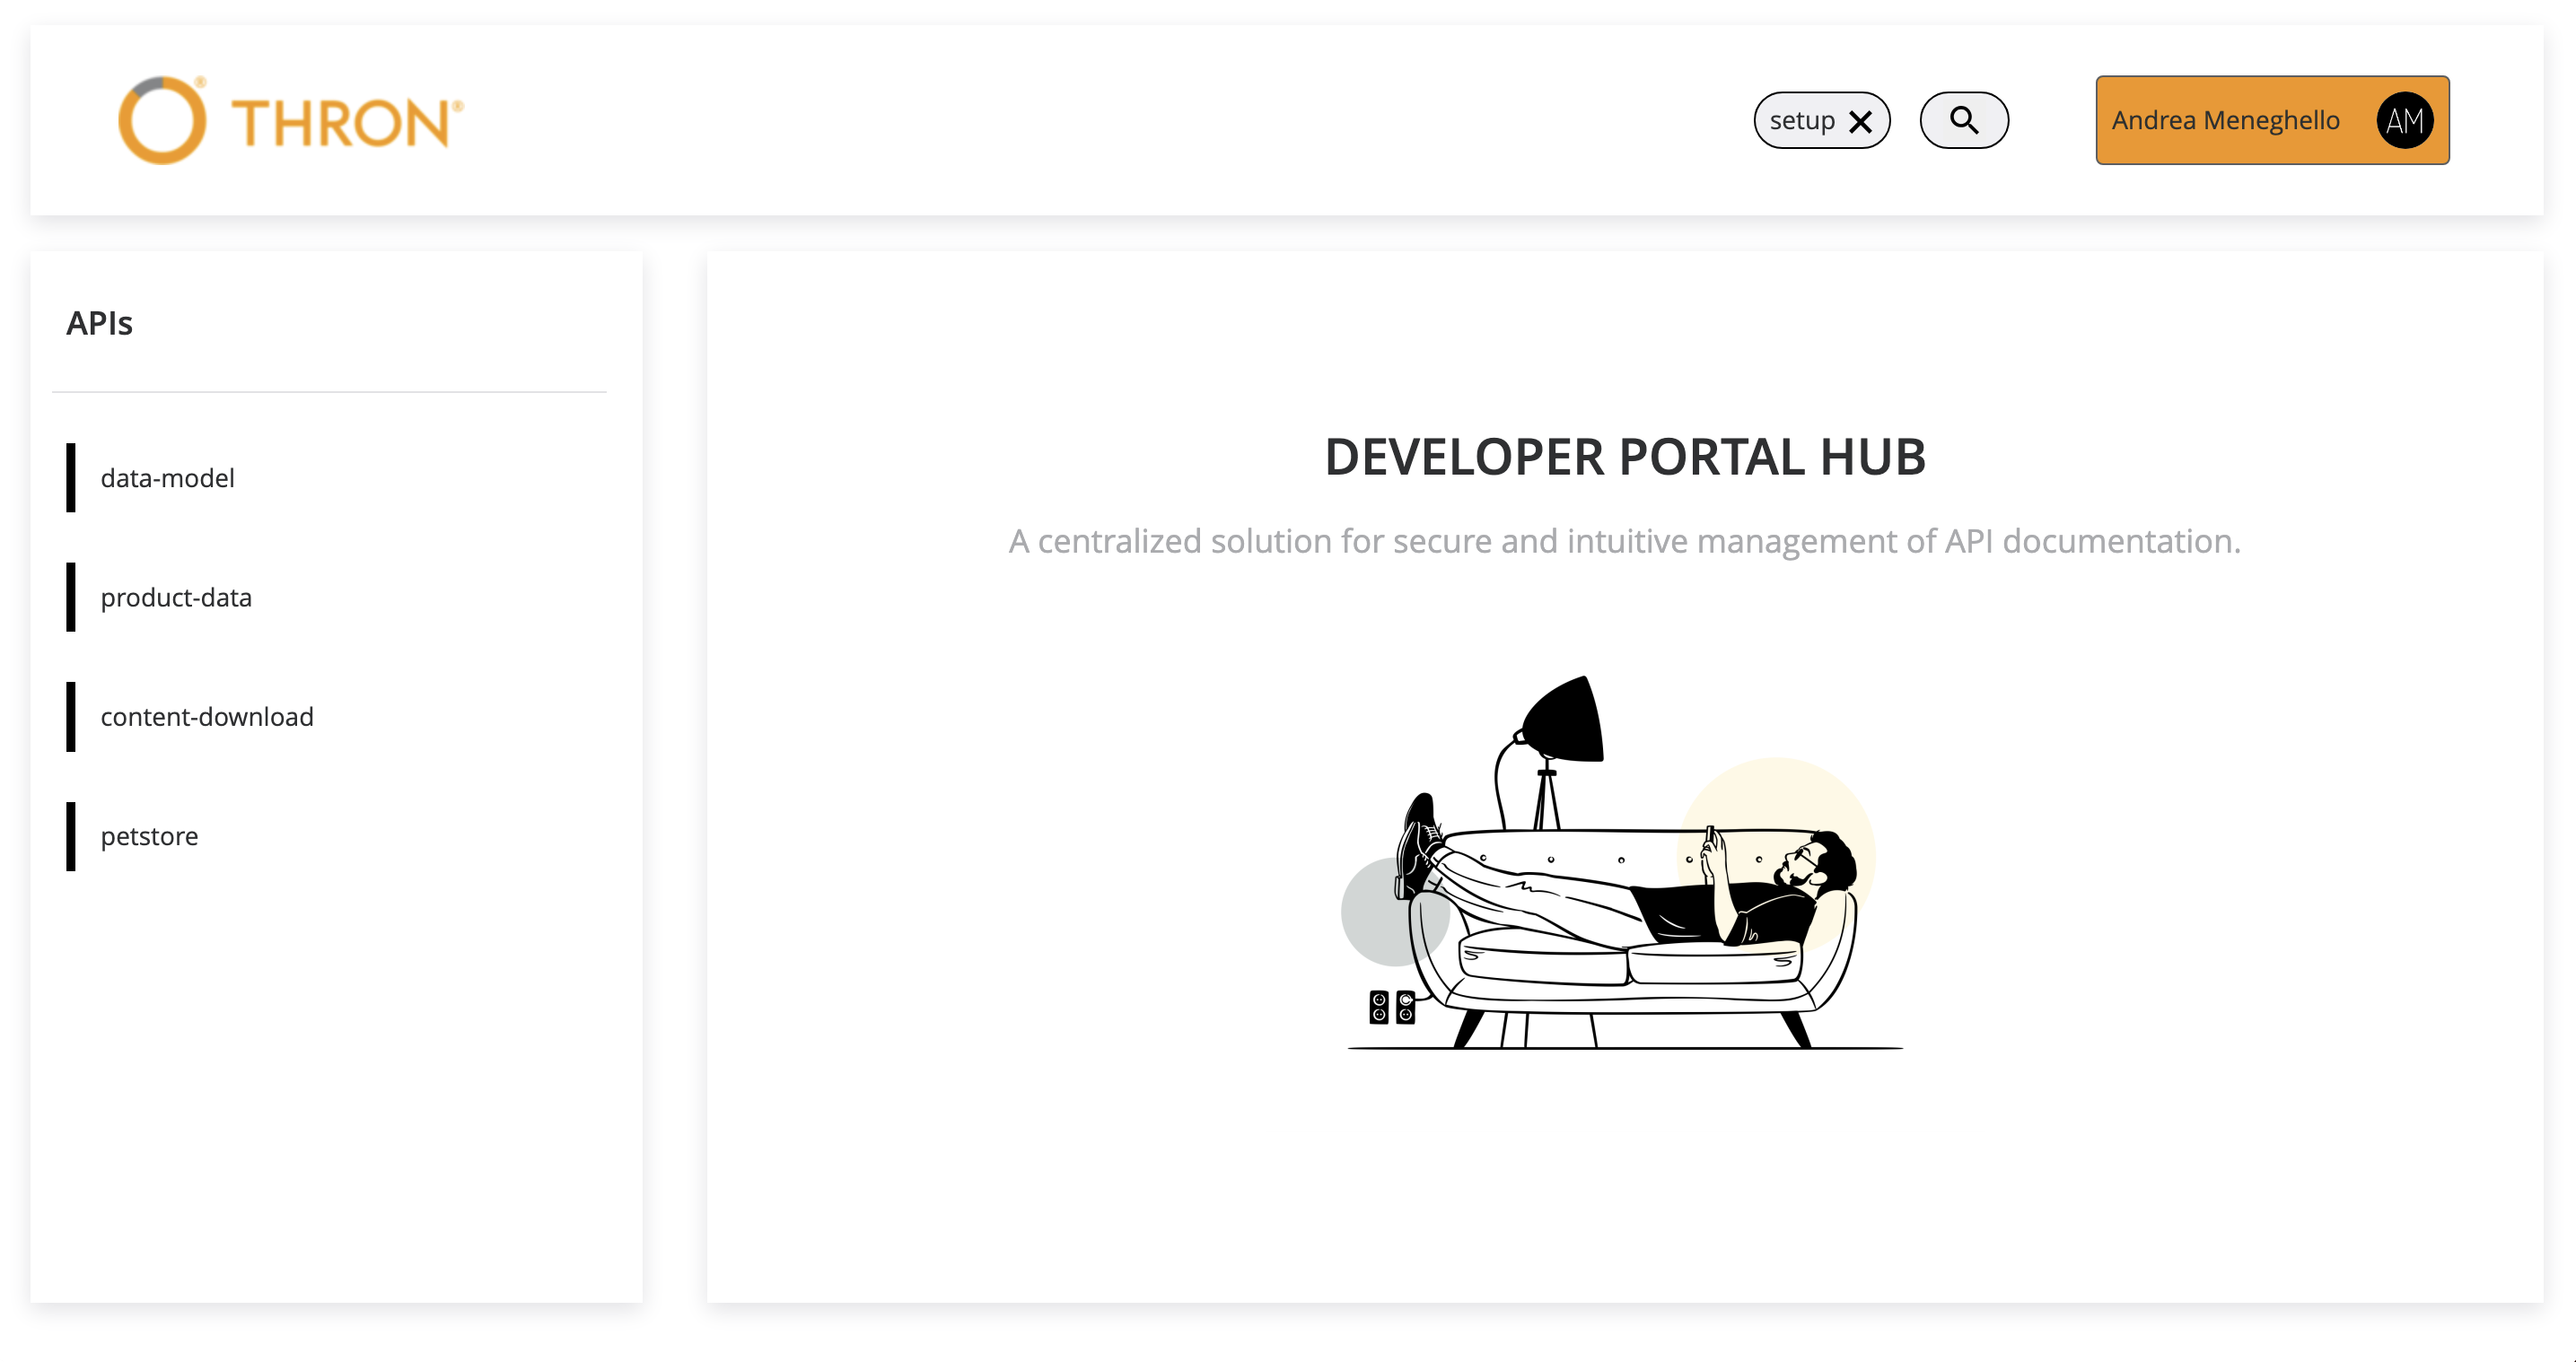
\includegraphics[width=0.6\textwidth, alt={Pagina principale dell'applicazione}]{images/frontend/HomeView.jpg}
  \caption{HomeView}\label{fig:home-view}
\end{figure}

Come la pagina di login, anche la pagina principale è stata sviluppata con un \textit{design responsive} (in figura~\ref{fig:home-view-responsive}).
Come si vede dall'immagine, si può notare che il menù laterale viene nascosto automaticamente e sarà accessibile cliccando l'apposito bottone a forma di \textit{hamburger}.

\begin{figure}[ht]
  \centering
  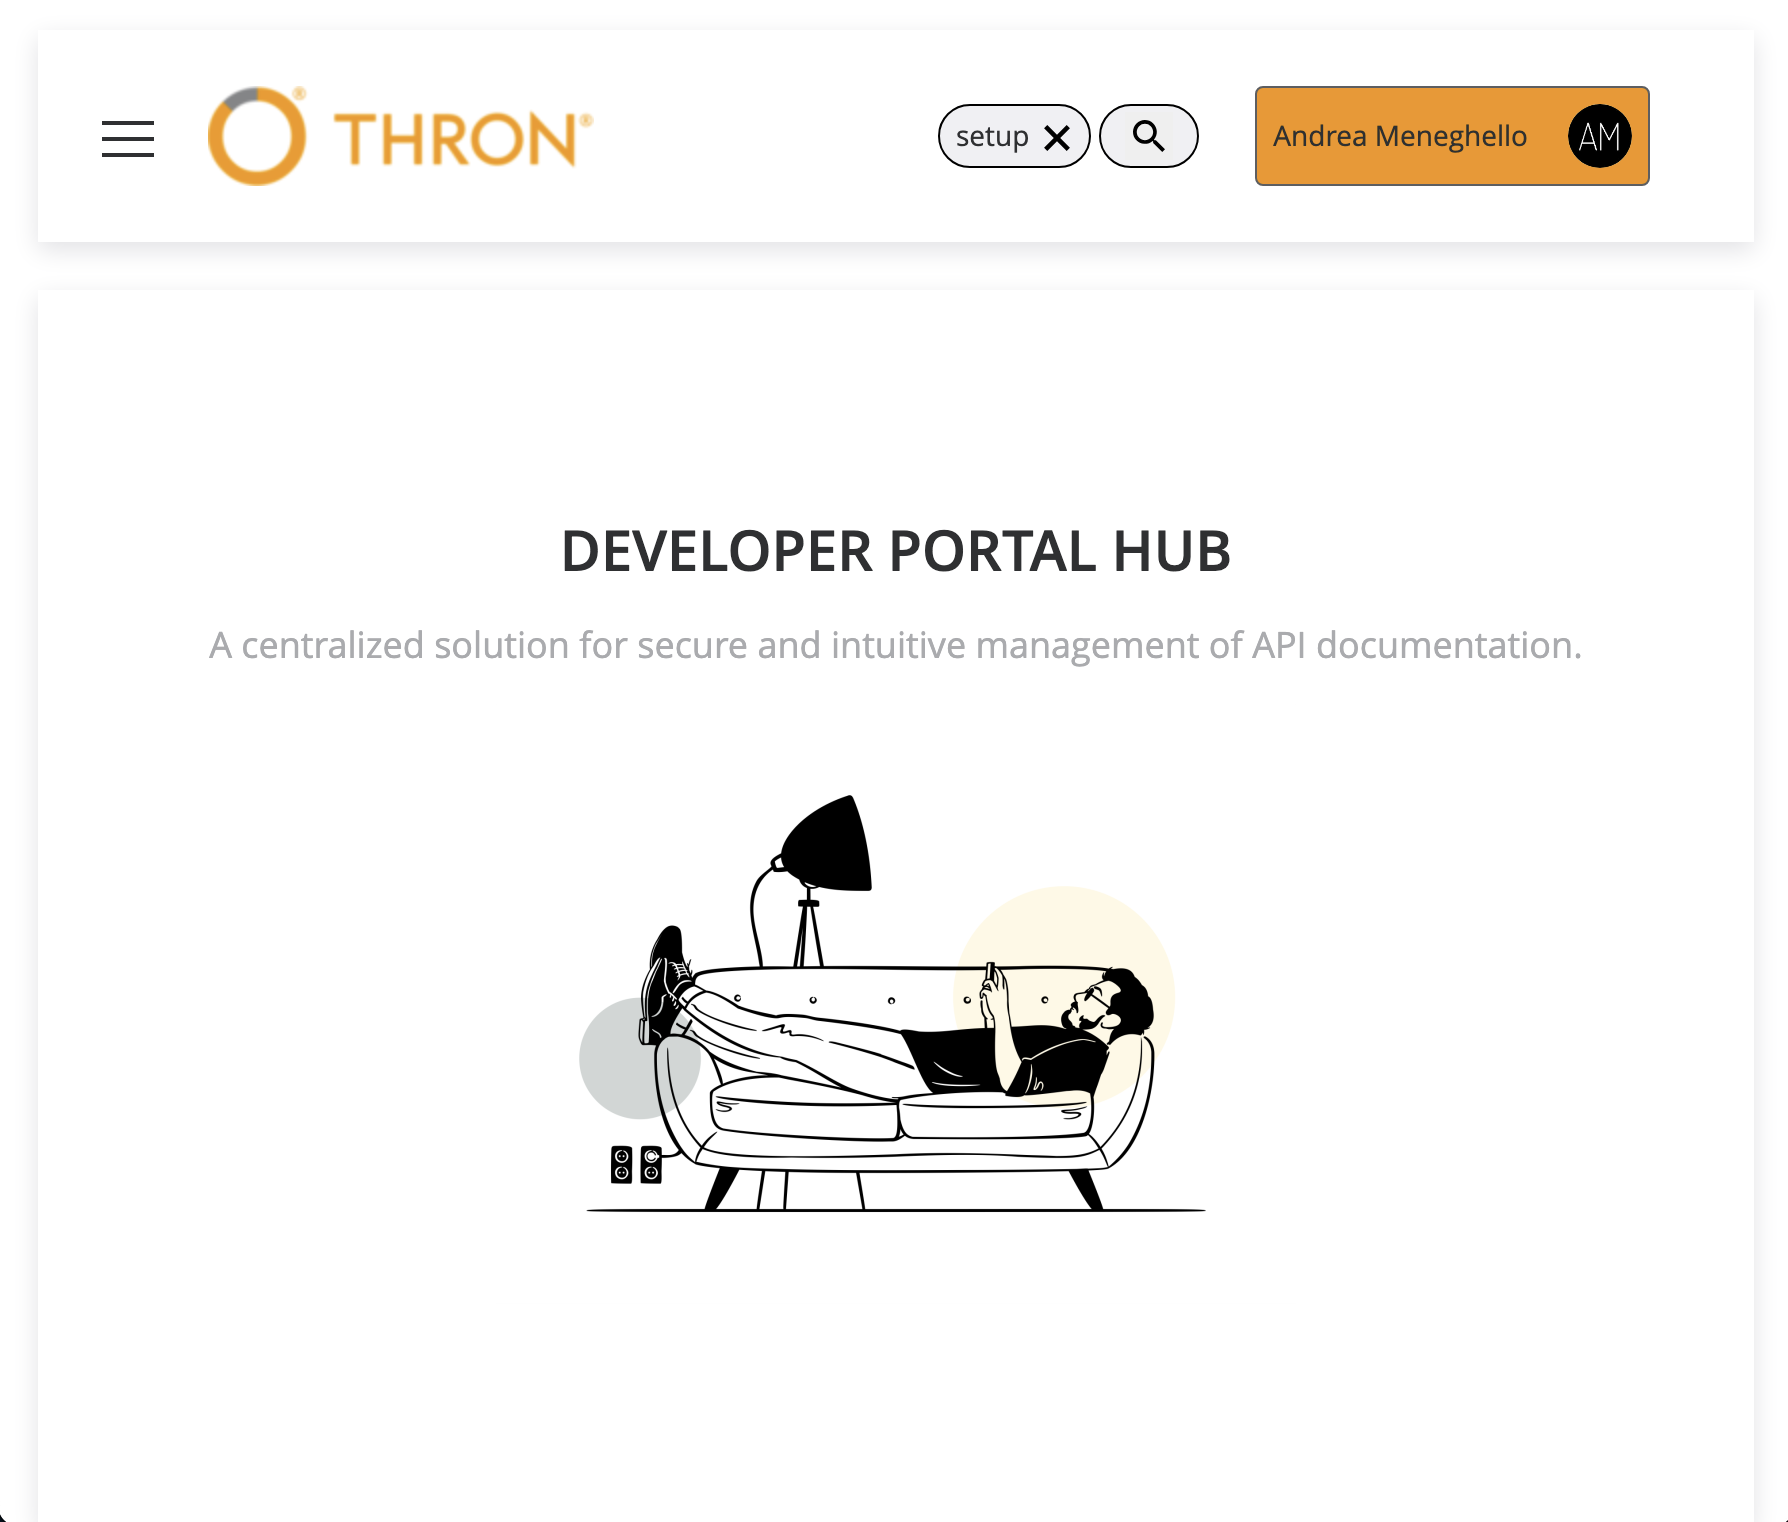
\includegraphics[width=0.5\textwidth, alt={Pagina principale responsive dell'applicazione}]{images/frontend/HomeViewRes.jpg}
  \caption{HomeView responsive}\label{fig:home-view-responsive}
\end{figure}


\subsubsection{NotFoundView}\label{subsubsec:not-found-view}
Quando un utente tenta di accedere ad una pagina non esistente, verrà reindirizzato automaticamente alla pagina di errore 404 (in figura~\ref{fig:not-found-view}).
La pagina consiste in un messaggio di errore con un'immagine, dove viene informato l'utente che la pagina richiesta non esiste.
Per tornare alla \textit{HomeView} basterà cliccare sul bottone \textit{Home} e si potrà continuare la navigazione all'interno del portale.

\begin{figure}[ht]
  \centering
  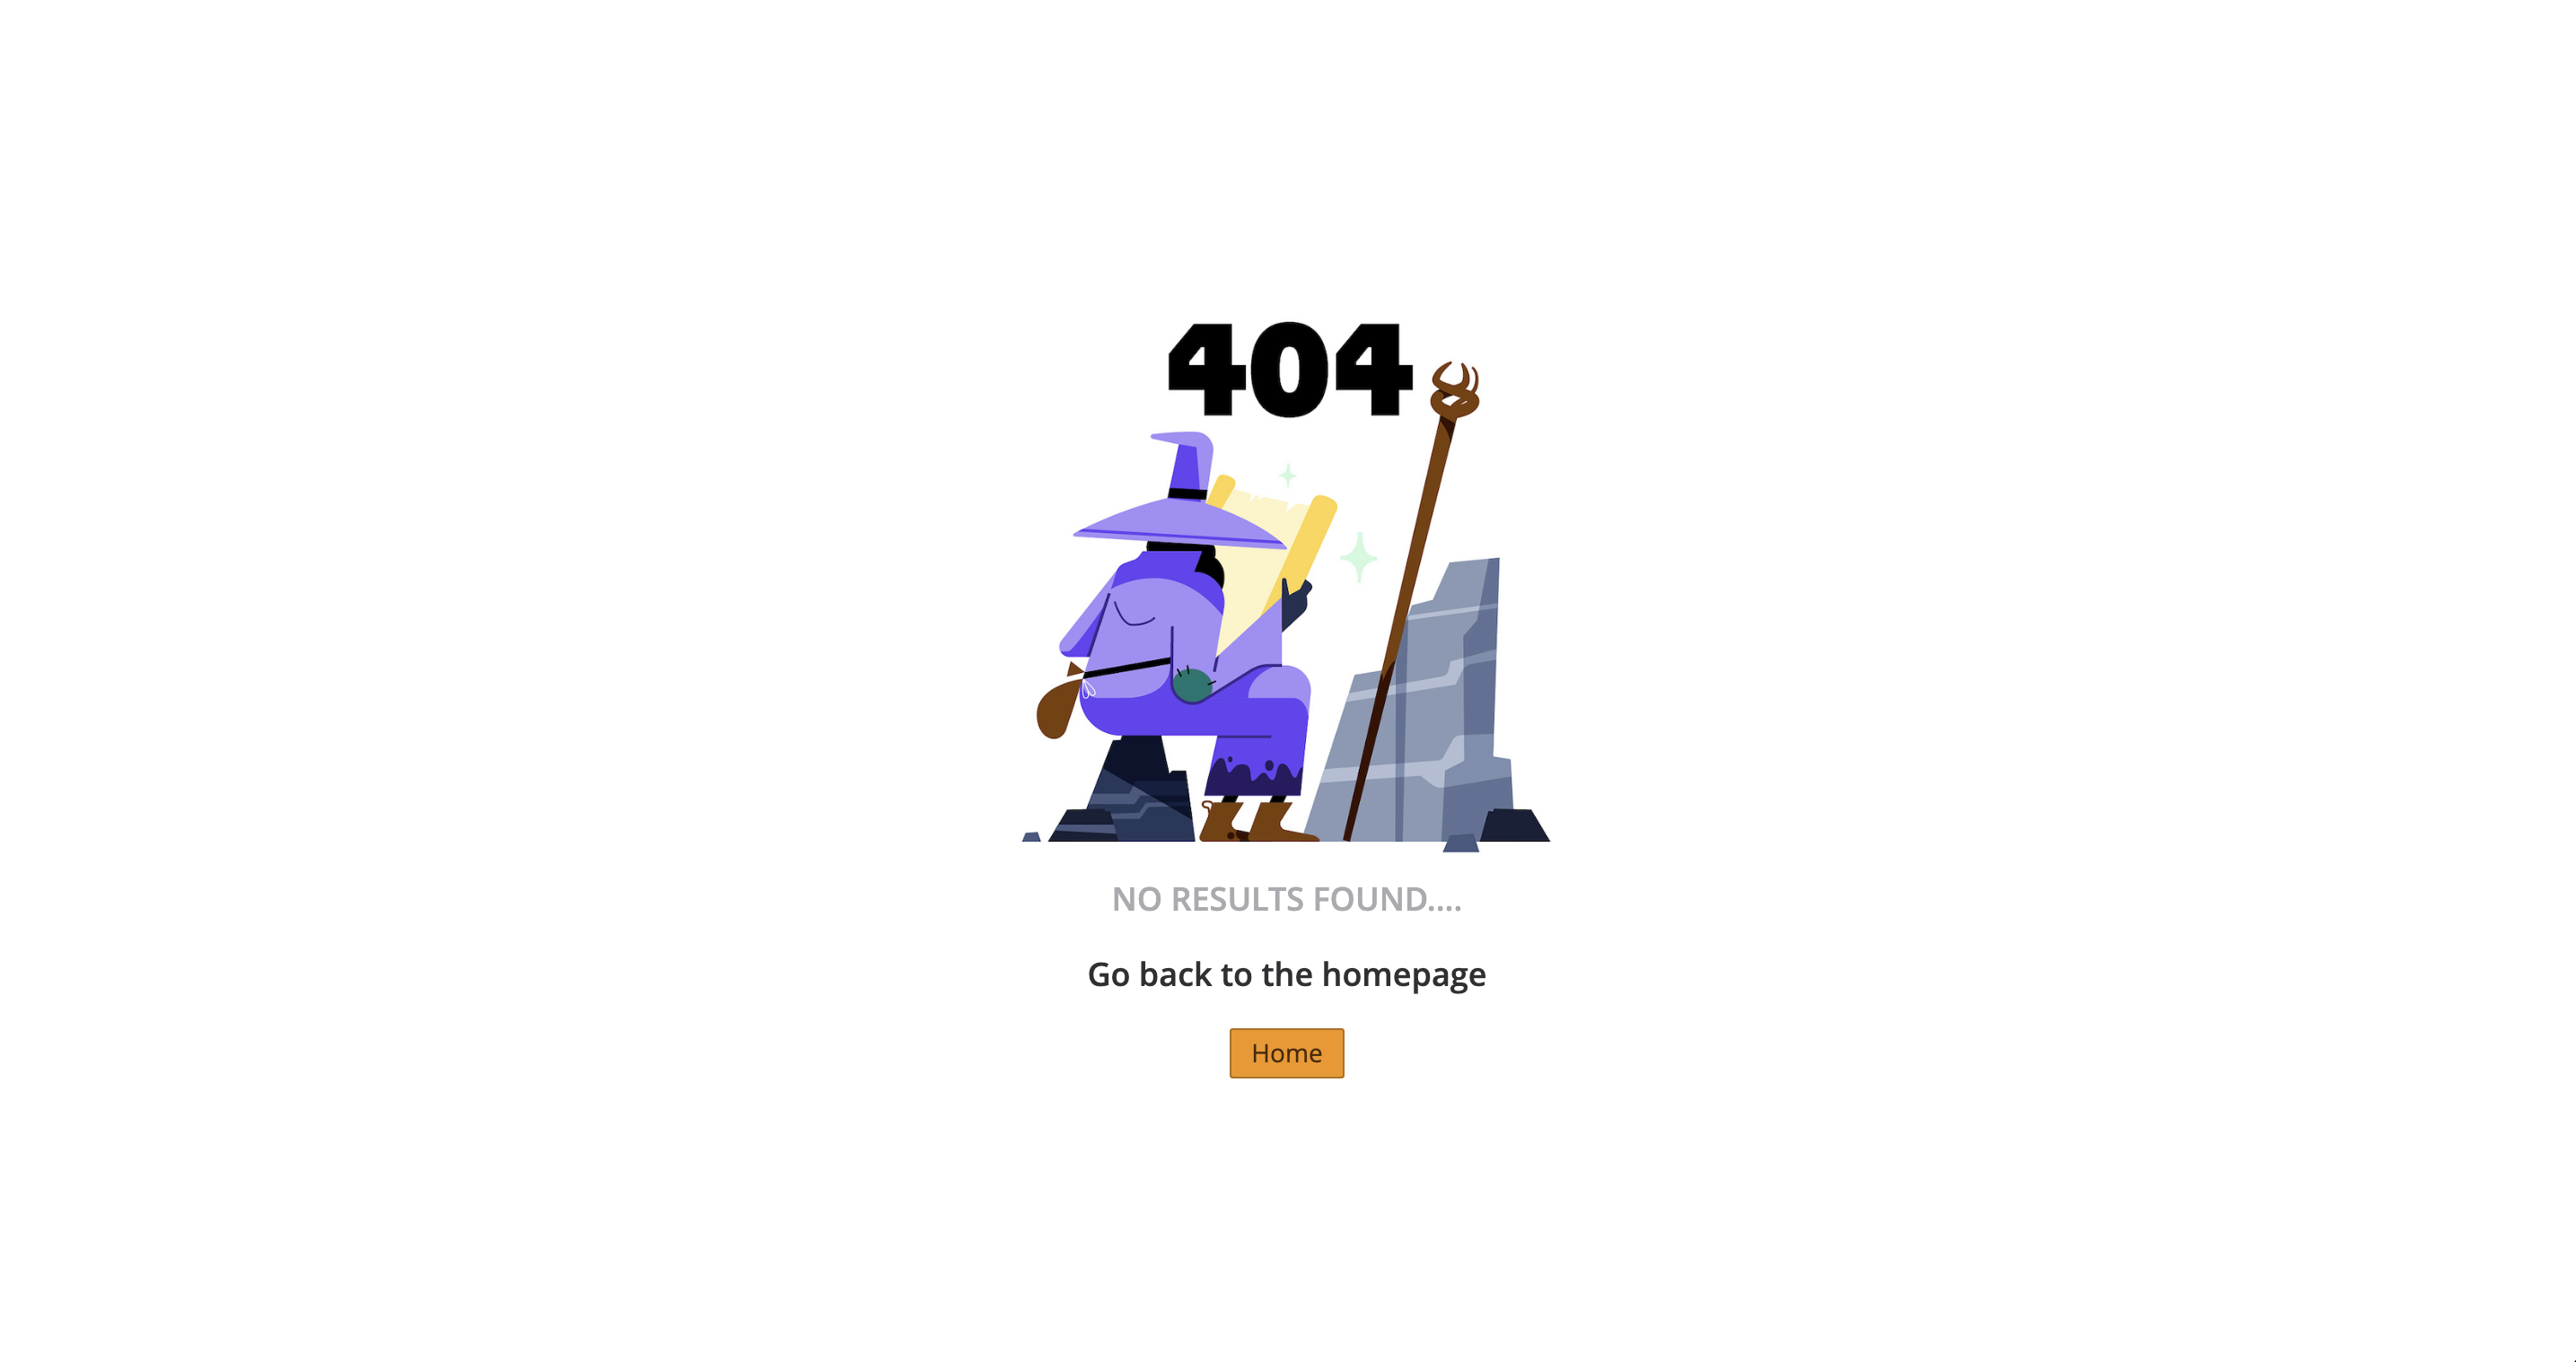
\includegraphics[width=0.6\textwidth, alt={Pagina di errore 404}]{images/frontend/NotFoundView.jpg}
  \caption{NotFoundView}\label{fig:not-found-view}
\end{figure}
\pagebreak
\subsection{Components}\label{subsec:components}

% Home
\subsubsection{HeaderNav}\label{subsubsec:header-nav}
Il componente rapppresenta la barra di navigazione superiore dell'applicazione (in figura~\ref{fig:header-nav-responsive}). Essa contiene il logo dell'applicazione, la \textit{chip} con il client-id
corrente, il bottone di ricerca e il \textit{popover} di logout. 
La barra viene sempre visualizzata una volta che l'utente ha effettuato il login all'interno del portale.\\
In caso di visualizzazione su schermi ridotti, l'\textit{HeaderNav} avrà un design responsive, dove viene aggiunto nell'estremità sinistra un bottone ad \textit{hamburger}
che permette di visualizzare la \textit{SideBar} a comparsa.

\begin{figure}[ht]
  \centering
  
\includegraphics[width=0.6\textwidth, alt={Barra di navigazione superiore con design responsive}]{images/frontend/HeaderRes.jpg}
  \caption{HeadearNav responsive}\label{fig:header-nav-responsive}
\end{figure}

\subsubsection{MainContent}\label{subsubsec:main-content}
Il componente rappresenta il contenuto principale dell'applicazione. Esso infatti contiene la struttura per visualizzare i dettagli di ogni API (in figura~\ref{fig:main-content}), tramite l'aiuto 
della libreria \textit{Swagger UI}.
La struttura segue il \textit{layout} di \textit{Swagger Editor} per motivi di semplicità e uniformità. Inizia con una descrizione iniziale, prosegue con la lista degli endpoint disponibili e conclude con l'elenco dei modelli.
I colori utilizzati sono uguali a quelli utilizzati in un comune \textit{Swagger Editor} per dare un senso di familiarità all'utente ed è stata una richiesta avanzata dal team.
Nell'angolo destro è stato aggiunto un bottone per il download della documentazione, che verrà discusso in seguito.
\begin{figure}[ht]
  \centering
  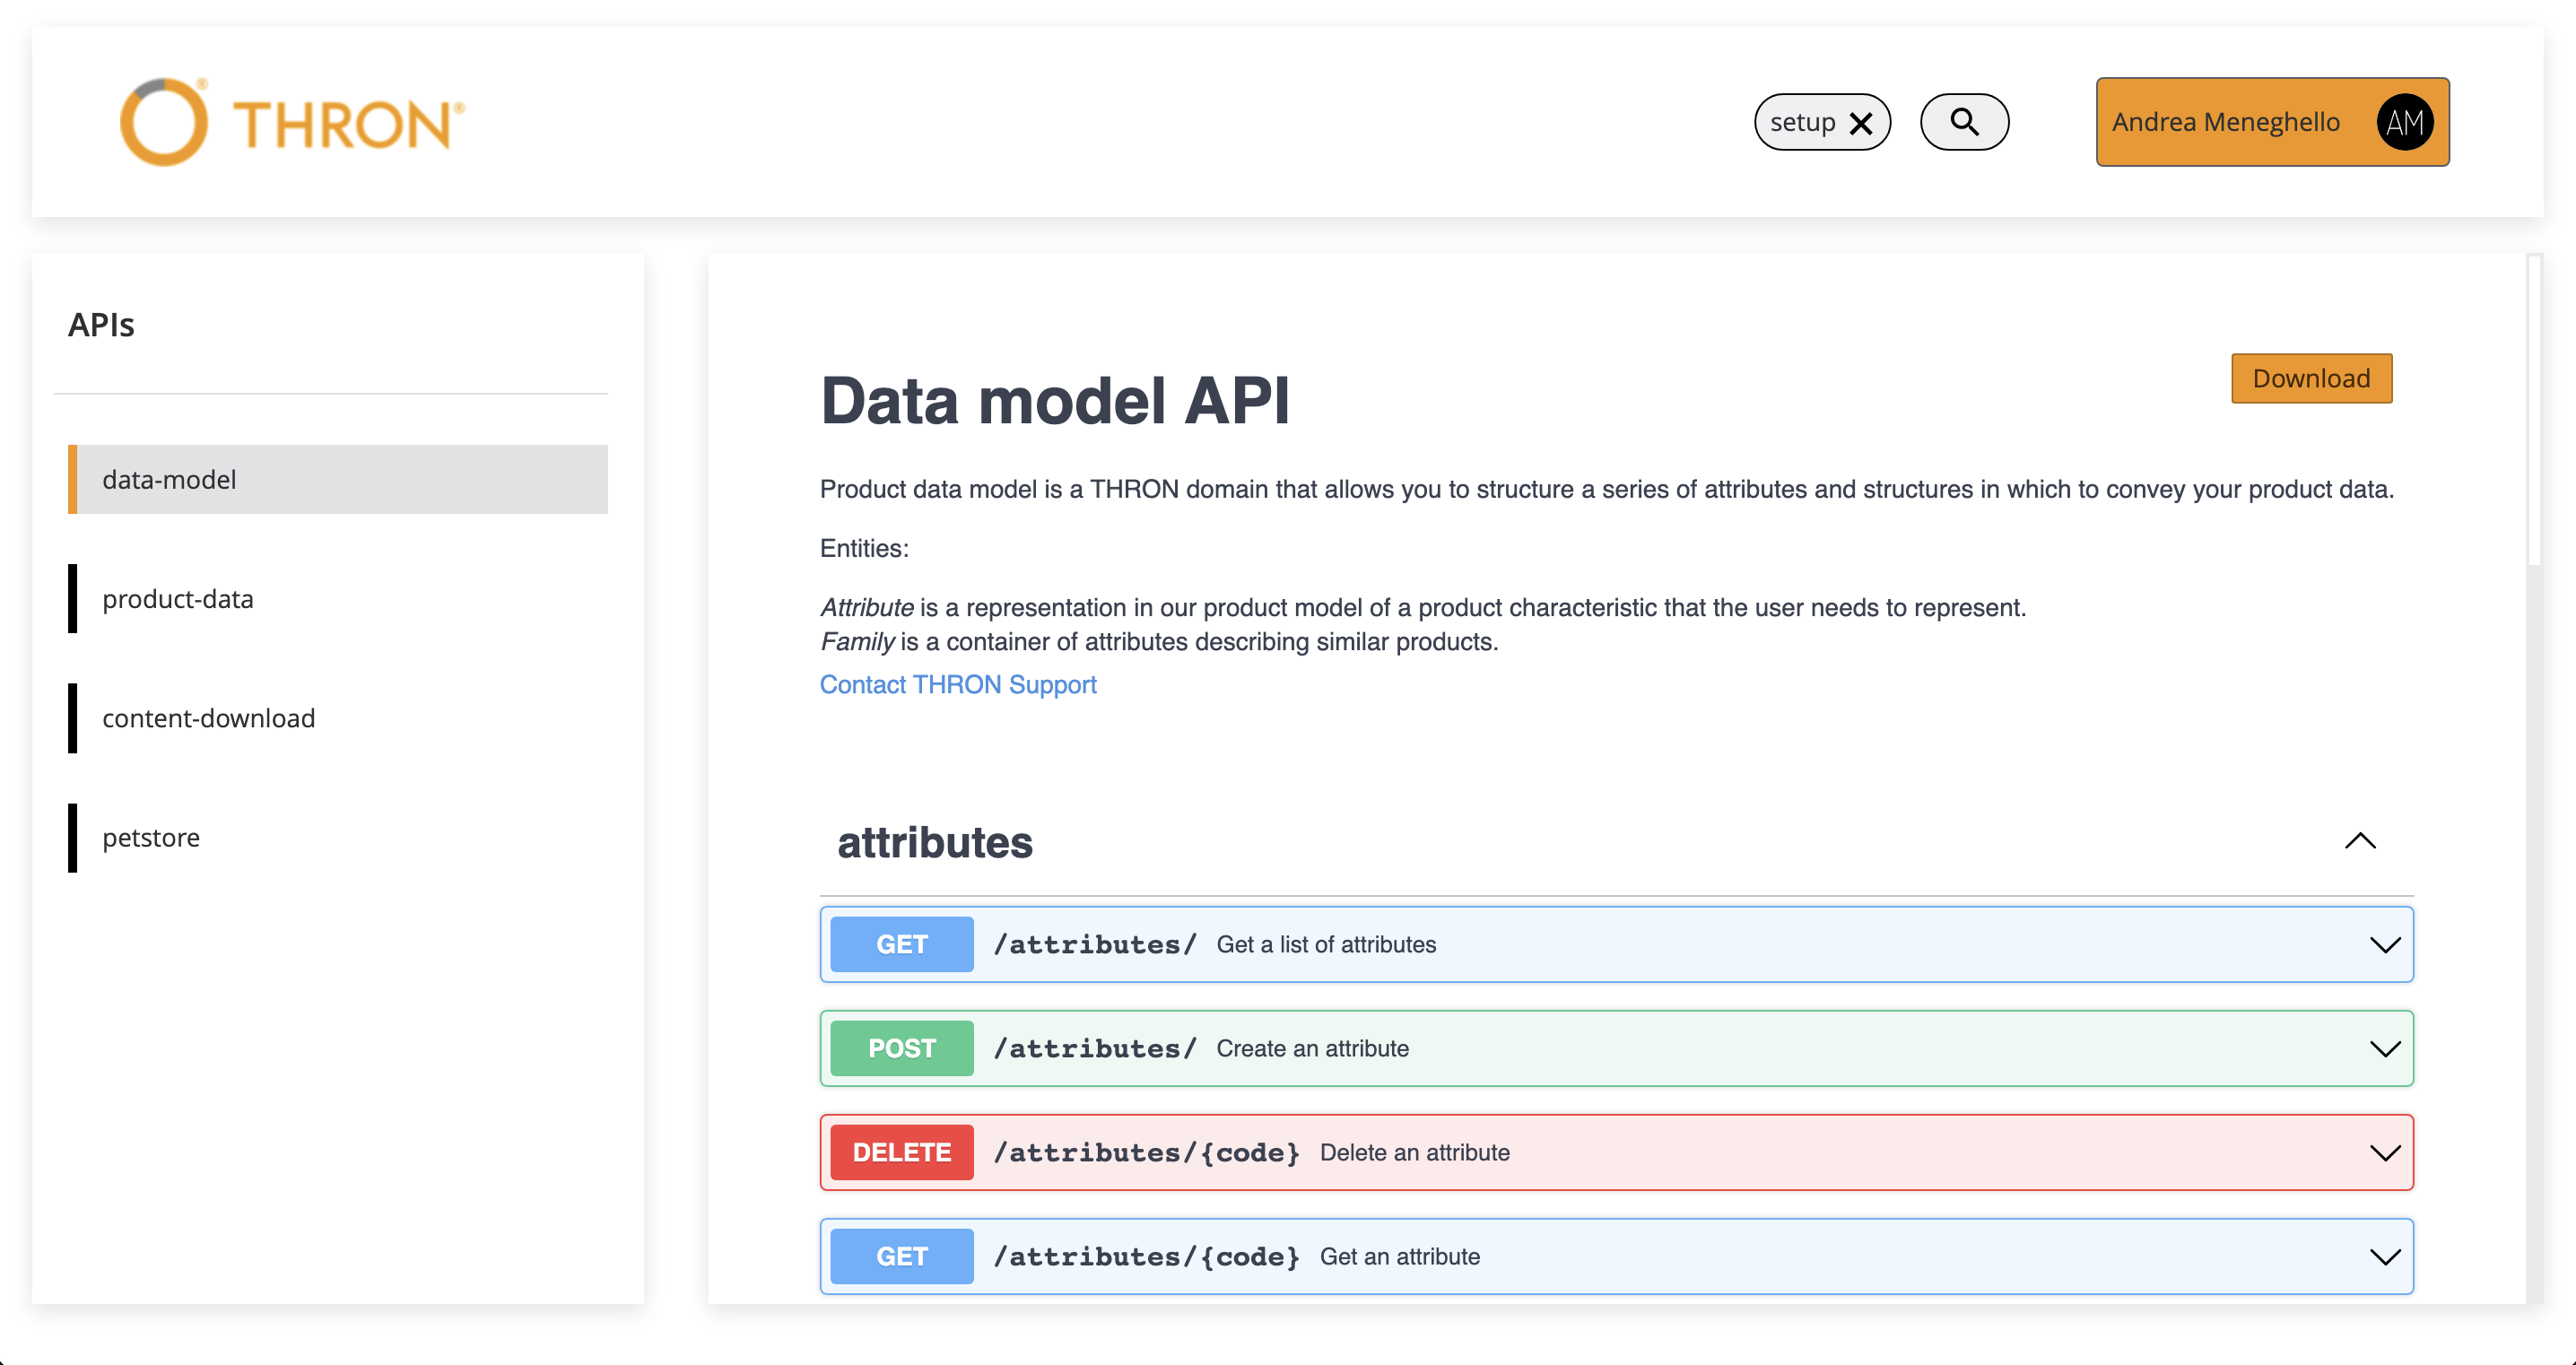
\includegraphics[width=0.6\textwidth, alt={Sezione per la visualizzazione dei dettagli di un API}]{images/frontend/DataModelView.jpg}
  \caption{MainContent}\label{fig:main-content}
\end{figure}
\pagebreak

Cliccando su uno degli endpoint disponibili, ci sarà una sezione dedicata per la visualizzazione dei dettagli di quest'ultimo (in figura~\ref{fig:try-it-out}).
I parametri e il \textit{Try it out} sono gestiti all'interno della \textit{utility SwaggerUtils} per una migliore suddivisione della logica.

\begin{figure}[ht]
  \centering
  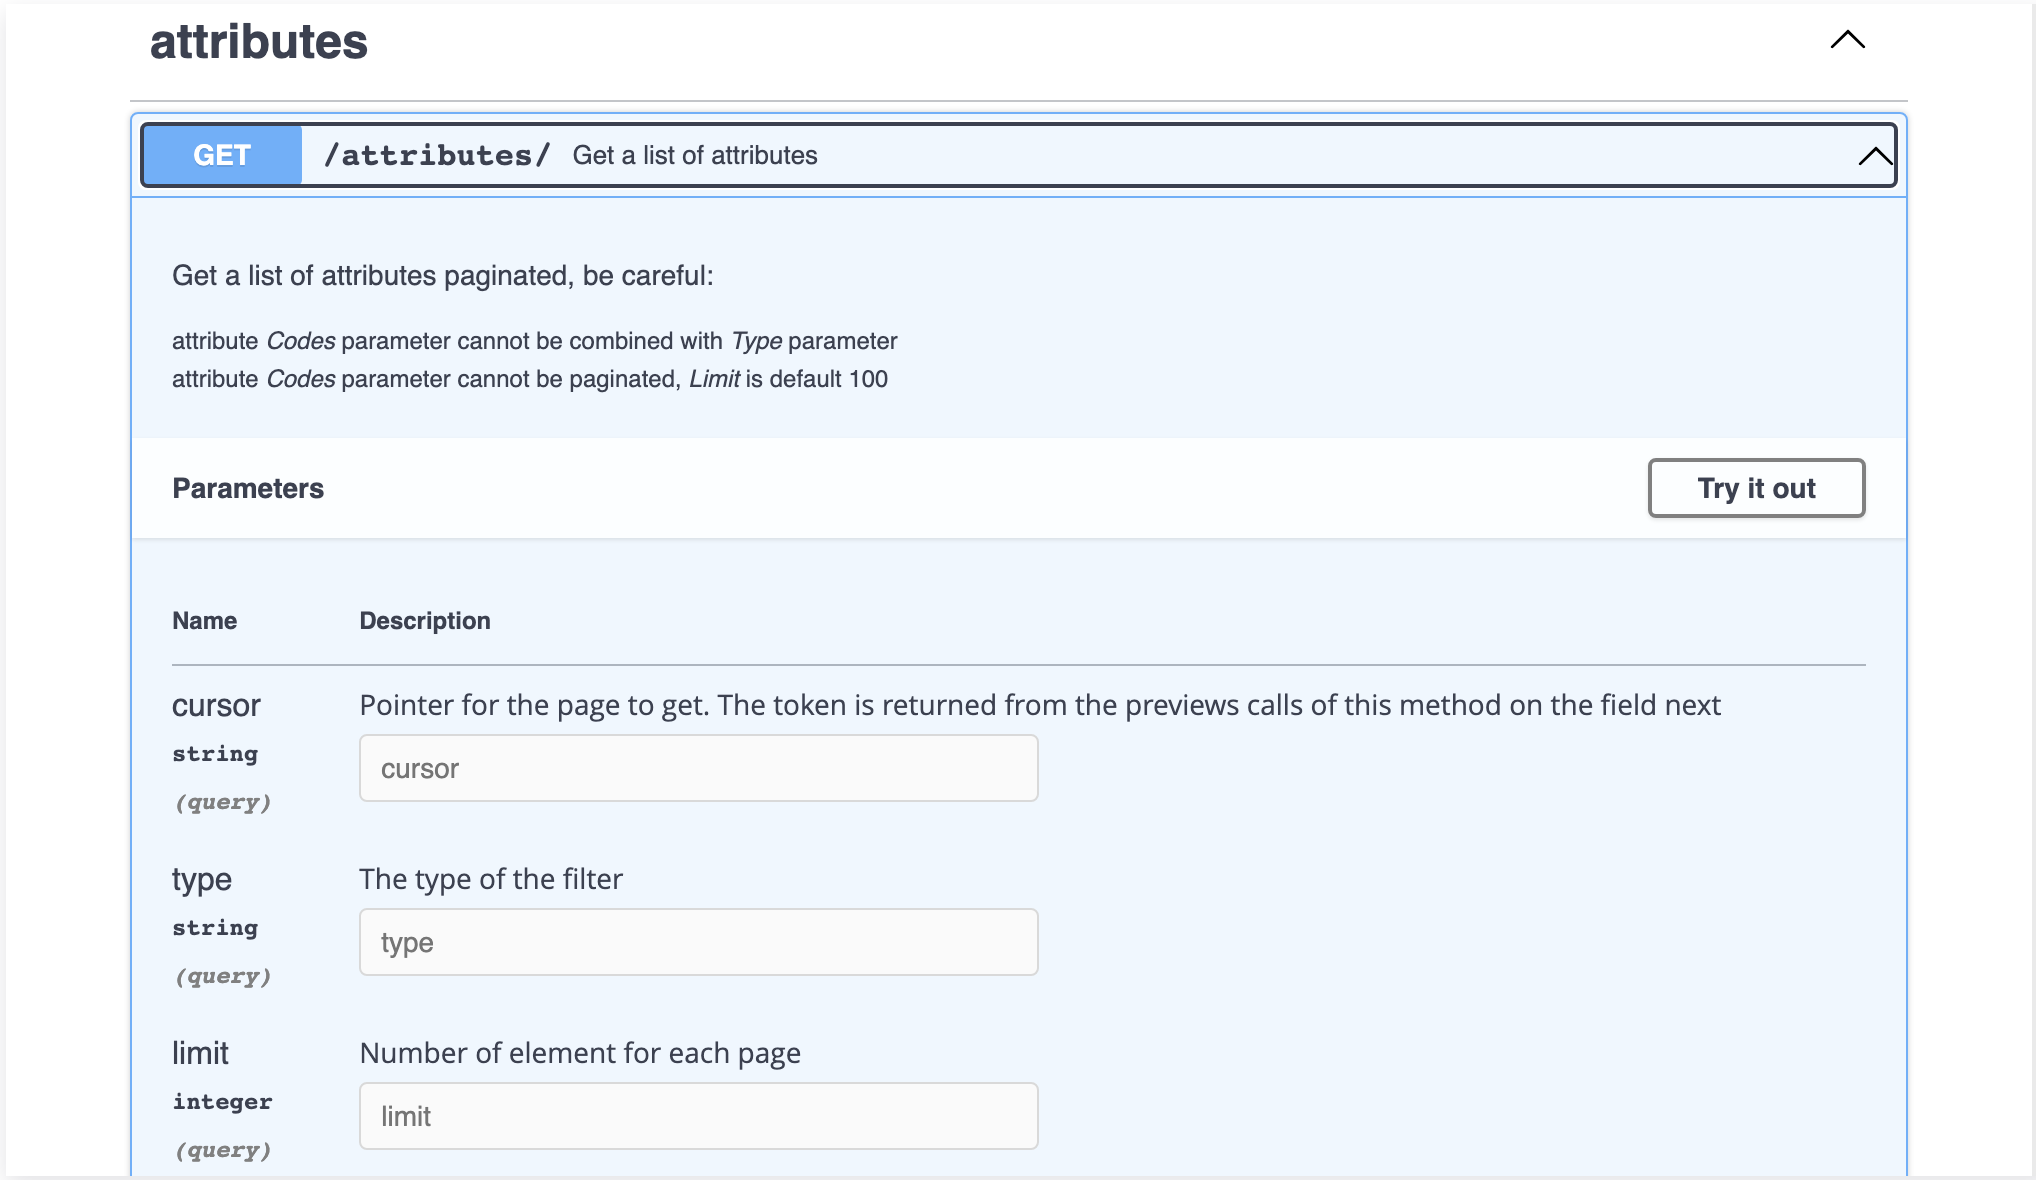
\includegraphics[width=0.6\textwidth, alt={Sezione try it out di un endpoint}]{images/frontend/TryItOut.jpg}
  \caption{Try it out di un endpoint}\label{fig:try-it-out}
\end{figure}

Inserendo i parametri e facendo quindi il \textit{try it out} verrà visualizzato il risultato della chiamata (in figura~\ref{fig:risposta-endpoint}).

\begin{figure}[ht]
  \centering
  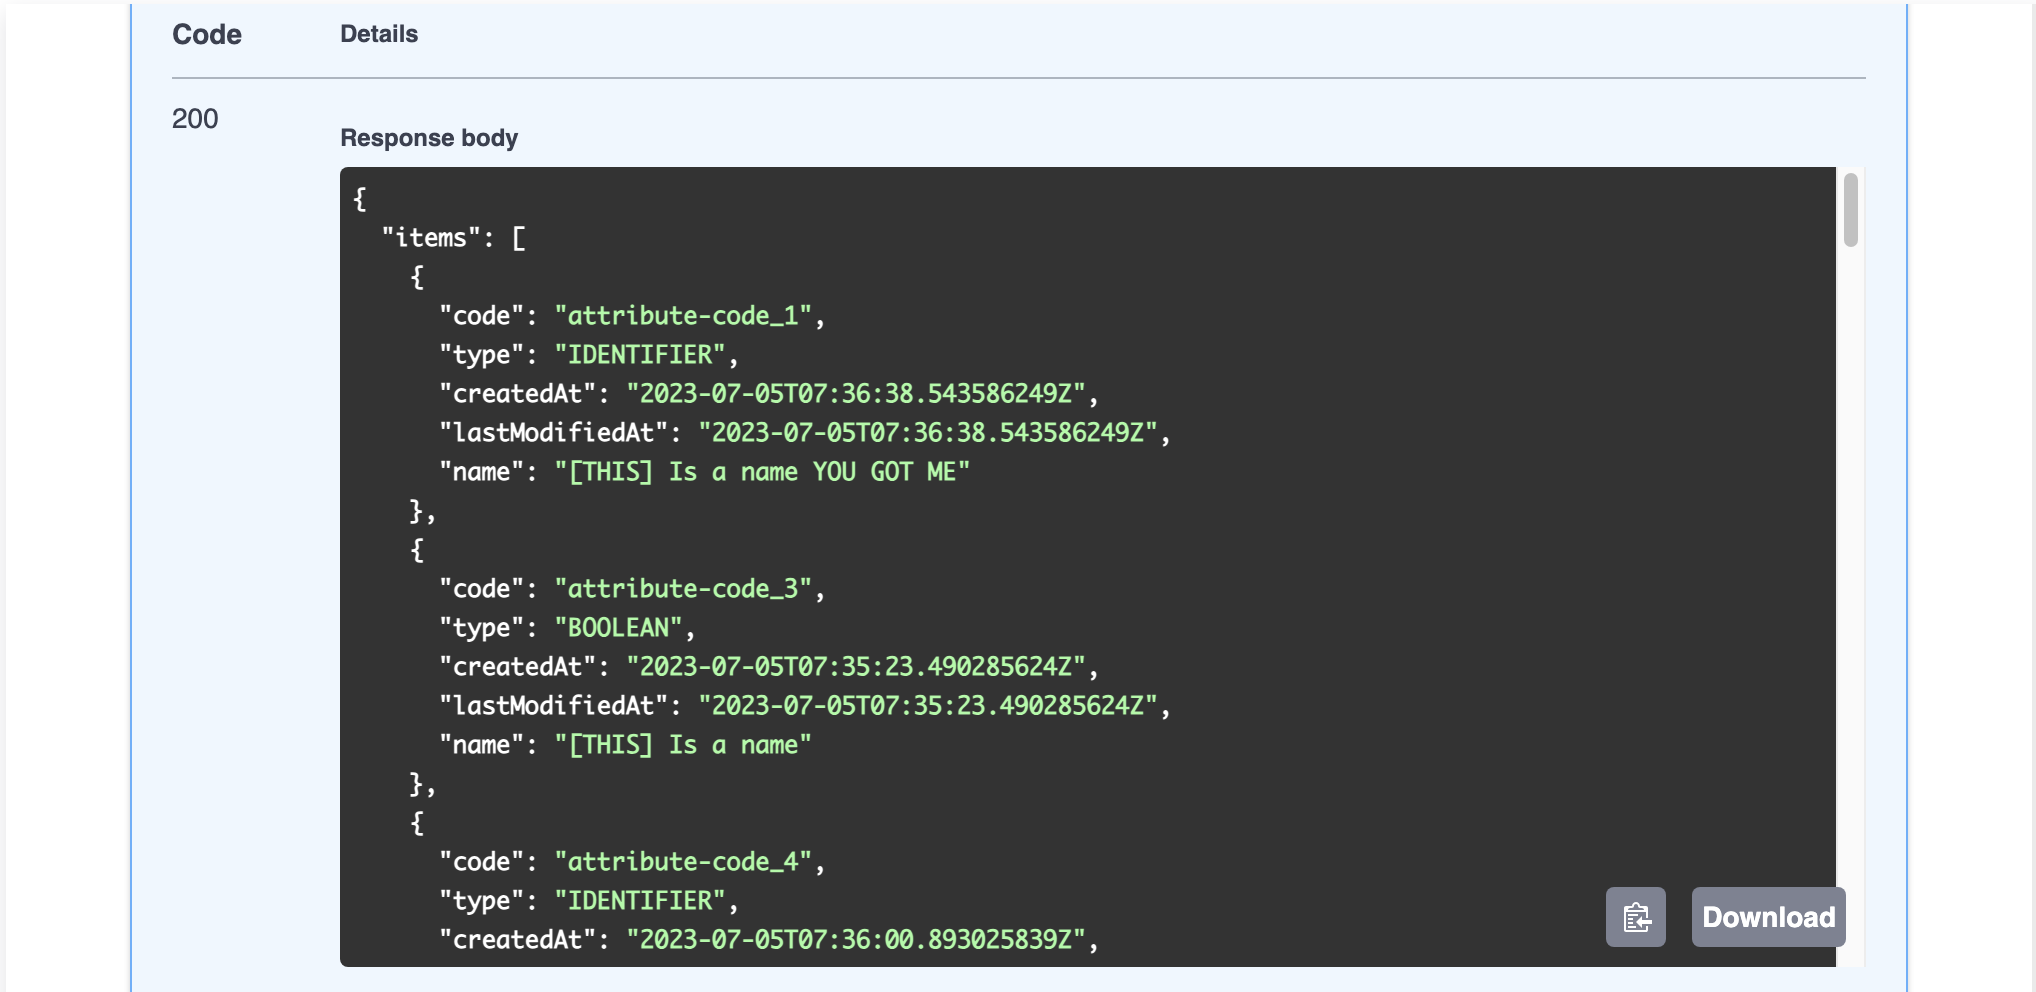
\includegraphics[width=0.6\textwidth, alt={Sezione per la visualizzazione della risposta di un endpoint}]{images/frontend/TryItOut3.jpg}
  \caption{Risposta di un endpoint}\label{fig:risposta-endpoint}
\end{figure}

Inoltre al di sotto sarà presente anche una lista delle possibili risposte che l'endpoint può restituire (in figura~\ref{fig:response-list}).

\begin{figure}[ht]
  \centering
  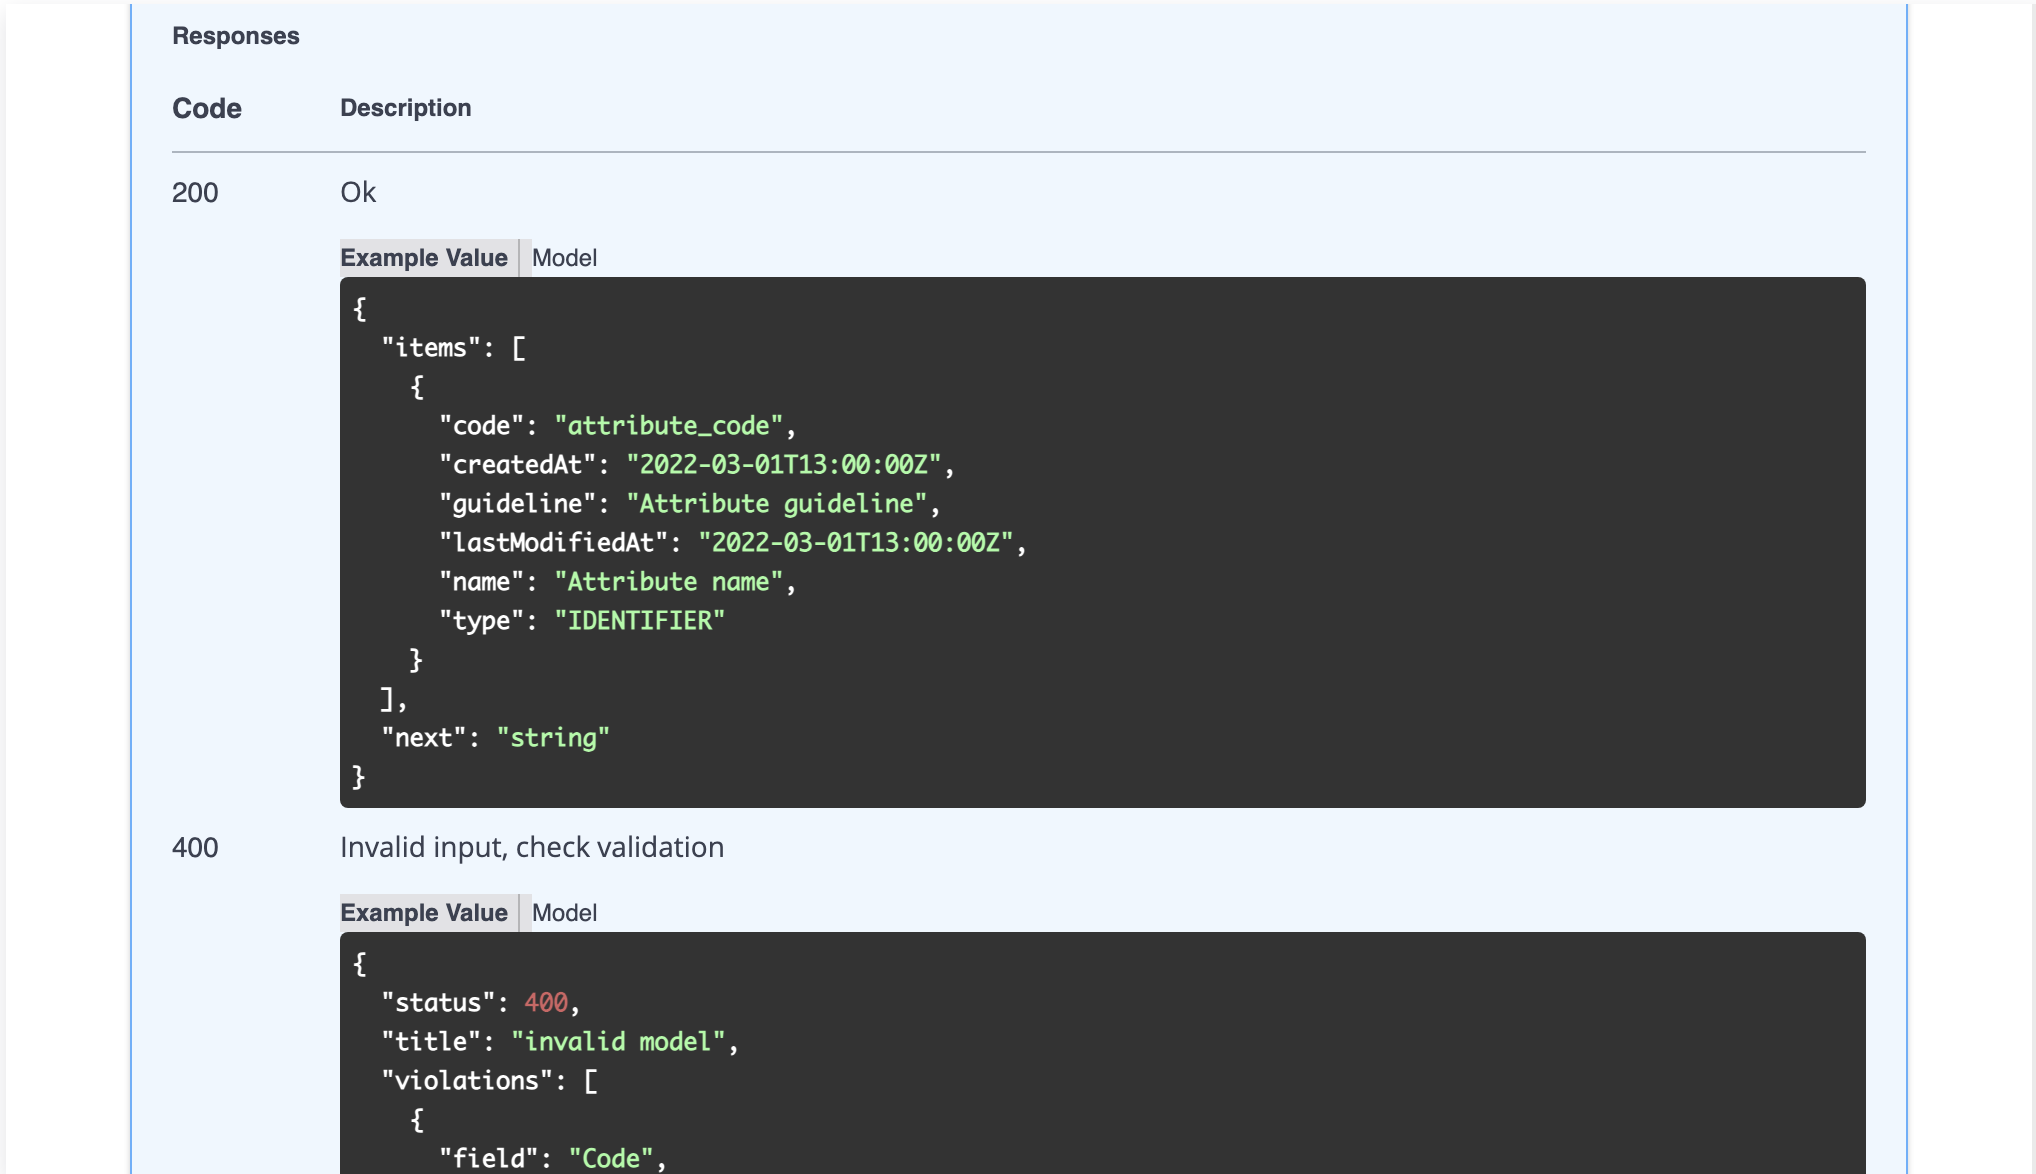
\includegraphics[width=0.6\textwidth, alt={Sezione per la visualizzazione delle possibili risposte di un endpoint}]{images/frontend/TryItOut4.jpg}
  \caption{Lista di risposte di un endpoint}\label{fig:response-list}
\end{figure}

\pagebreak

Nel caso di chiamate con necessità del parametro \textit{client-id}, è stato gestito tramite l'\textit{utility SwaggerUtils} l'\textit{autofill} di esso.
Infatti, il campo verrà compilato con il \textit{client-id} presente nella \textit{chip}, evitando che si inseriscano valori non presenti per 
quell'ambiente di sviluppo.


\subsubsection{SideBar}\label{subsubsec:side-bar}
Il componente rappresenta la barra di navigazione laterale dell'applicazione che contiene la lista di tutte le API disponibili nel portale (in figura~\ref{fig:side-bar-responsive}).
Attraverso la barra sarà possibile navigare tra le varie API, andando a visualizzare i dettagli di ognuna di esse. 
Il componente è stato sviluppato utilizzando un design responsive, che permette di visualizzare il contenuto in maniera ottimale anche su spazi ridotti, 
infatti il menù andrà a nascondersi automaticamente e sarà accessibile cliccando l'apposito bottone a forma di \textit{hamburger} situato nell'\textit{HeaderNav}.\\

\begin{figure}[ht]
  \centering
  \includegraphics[width=0.5\textwidth, alt={Design responsive della barra laterale}]{images/frontend/Sidebar.jpg}
  \caption{Design responsive SideBar}\label{fig:side-bar-responsive}
\end{figure}

\subsubsection{StartPage}\label{subsubsec:start-page}
% \gls{apig} è un portale che permette di consultare la documentazione delle API disponibili nel sistema.
Il componente rappresenta la pagina iniziale di benvenuto dell'applicazione ed è la prima schermata che l'utente visualizza dopo aver effettuato il login con successo.
Essa contiene il nome del portale, una breve descrizione e un'immagine. Per iniziare la navigazione nel portale, basterà usare la \textit{SideBar}.

\subsubsection{SwaggerLoader}\label{subsubsec:swagger-loader}
Il componente rappresenta il loader di caricamento per il \textit{MainContent} (in figura~\ref{fig:swagger-loader}). 
Esso rappresenta un caricamento di stile \textit{skeleton}, ovvero un caricamento di contenuto che simula il contenuto finale, mentre questo viene caricato, attraverso un sfondo dinamico grigio.
Il componente ha la stessa struttura del \textit{MainContent}, quindi segue lo stesso design responsive.
Il loader sarà visibile ogni volta che l'utente clicca su una delle API disponibili nella \textit{SideBar}, e scomparirà una volta che il contenuto sarà caricato correttamente.

\begin{figure}[ht]
  \centering
  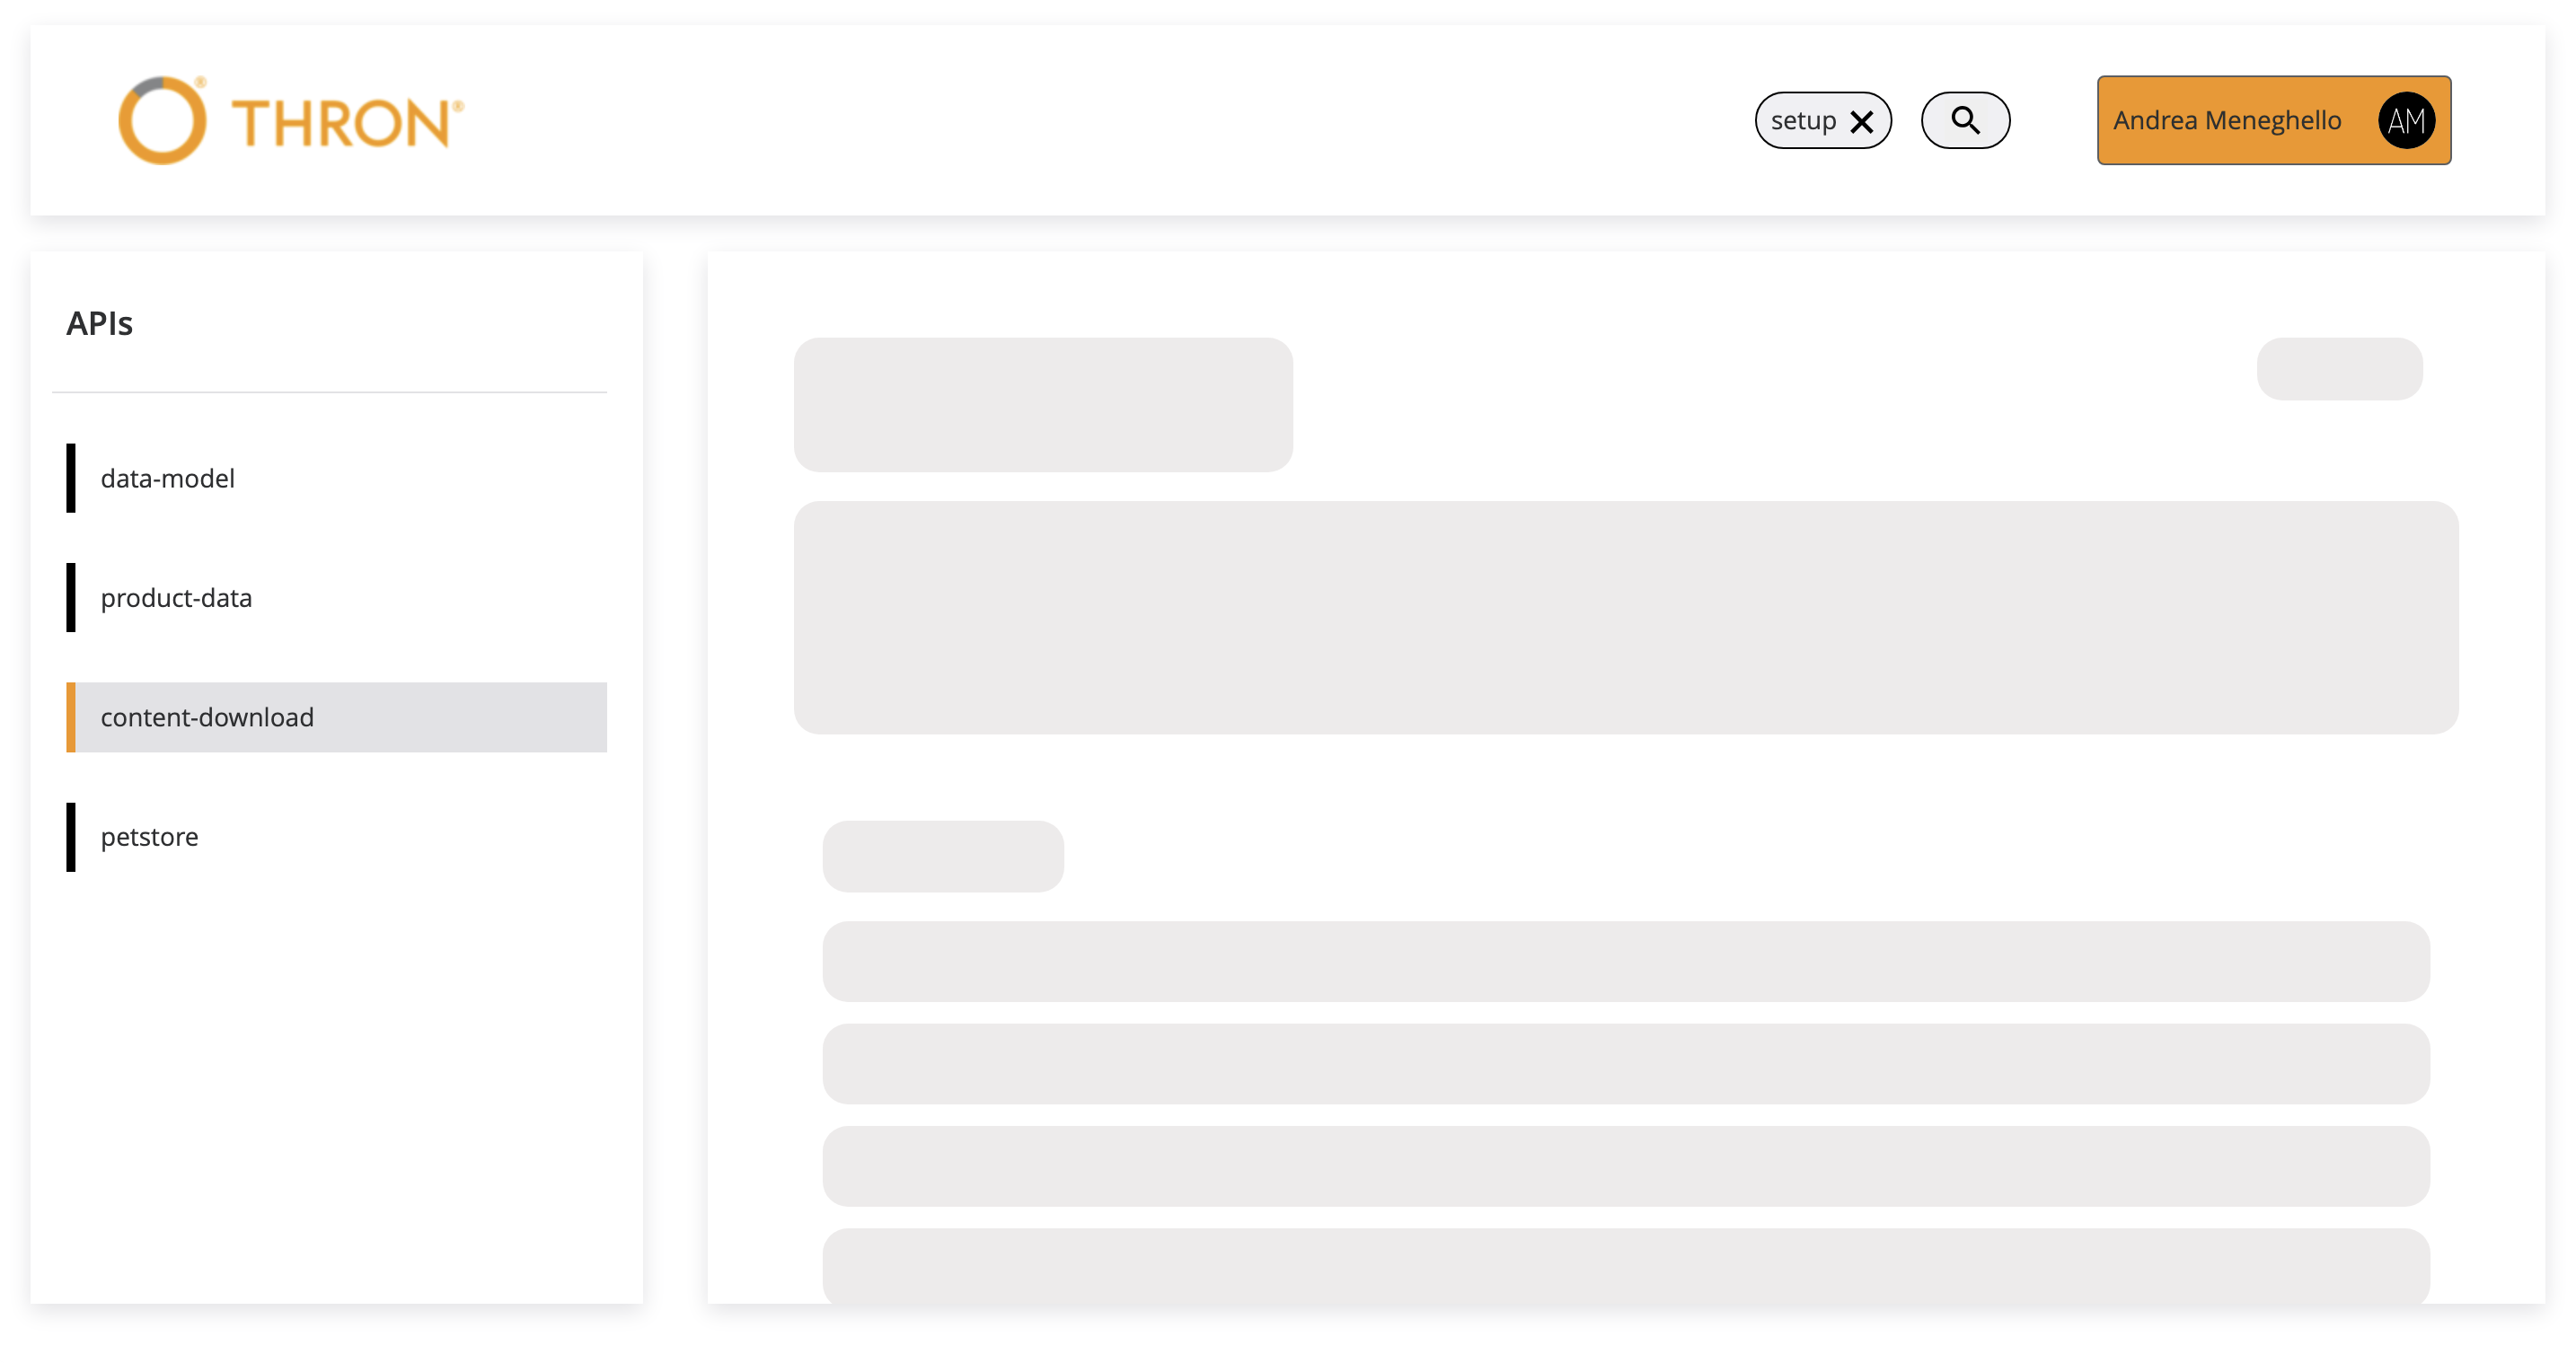
\includegraphics[width=0.6\textwidth, alt={Skeleton loader di caricamento per contenuto principale}]{images/frontend/SwaggerLoader.jpg}
  \caption{SwaggerLoader}\label{fig:swagger-loader}
\end{figure}

% \pagebreak
\subsubsection{DownloadButton}\label{subsubsec:download-button}
Il componente rappresenta il bottone di download presente in ogni pagina di dettaglio dell'API specifica. Esso è stato sviluppato rispettando il \textit{design system}
aziendale, infatti non è un componente \textit{custom} creato da zero, ma è stato sviluppato utilizzando il componente \textit{Button} della libreria \textit{Components} THRON.
Il componente da la possibilità di scegliere la grandezza, il testo del bottone e icone da visualizzare.
Il componente permette all'utente di scaricare la documentazione dell'API in formato \textit{.yaml}, con un nome predefinito a seconda 
del servizio scaricato. Una volta cliccato, andrà ad aprire una finestra secondaria del browser, e il file verrà scaricato automaticamente.\\

\subsubsection{LogoutButton}\label{subsubsec:logout-button}
Il componente rappresenta il bottone di logout presente nella barra di navigazione superiore 
dell'applicazione ed è stato sviluppato rispettando il \textit{design system} 
aziendale, infatti utilizza la libreria \textit{THRON Components}.
Nello specifico è stato chiamato bottone per comodità, ma in realtà si tratta di un \textit{popover}, ovvero un componente a tendina che si apre
tramite l'\textit{hover} del mouse. Esso permette all'utente di effettuare il logout dal portale tramite un \textit{popup}, con successivo reindirizzamento
alla pagina di login.

%aggiungere foto hover

% Login
\subsubsection{LoginButton}\label{subsubsec:login-button}
Il componente rappresenta il bottone di accesso al portale presente nella pagina di login dell'applicazione. Esso è stato sviluppato rispettando il \textit{design system} aziendale.
Il seguente bottone aprirà un \textit{popup} dove sarà possibile inserire le credenziali (e-mail e password) per effettuare l'accesso tramite \textit{Microsoft} 365.
Una volta effettuato il login, l'utente verrà reindirizzato alla pagina principale del portale.

% Components
\subsubsection{SearchButton}\label{subsubsec:search-button}
Il componente rappresenta il bottone di ricerca presente nella barra di navigazione superiore dell'applicazione.
Si tratta di un componente \textit{custom} creato da me, utilizzato per aprire la barra di ricerca globale del portale. 

\subsubsection{SearchBar}\label{subsubsec:search-bar}
Il componente rappresenta la barra di ricerca globale dell'applicazione (in figura~\ref{fig:search-bar}). 
Essa consiste in una barra dove poter inserire il \textit{client-id} o il nome dell'\textit{API} da cercare,
con un'icona di ricerca a fianco. Per una migliore esperienza di ricerca, è necessario utilizzare il componente insieme al componente \textit{autocomplete} descritto in seguito.
Infatti i componenti insieme, costituiscono la ricerca all'interno del portale. Inoltre La \textit{SearchBar} è accessibile anche tramite tastiera,
infatti tramite il comando \textit{Ctrl + B} sarà possibile aprire la barra di ricerca.\\

\begin{figure}[ht]
  \centering
  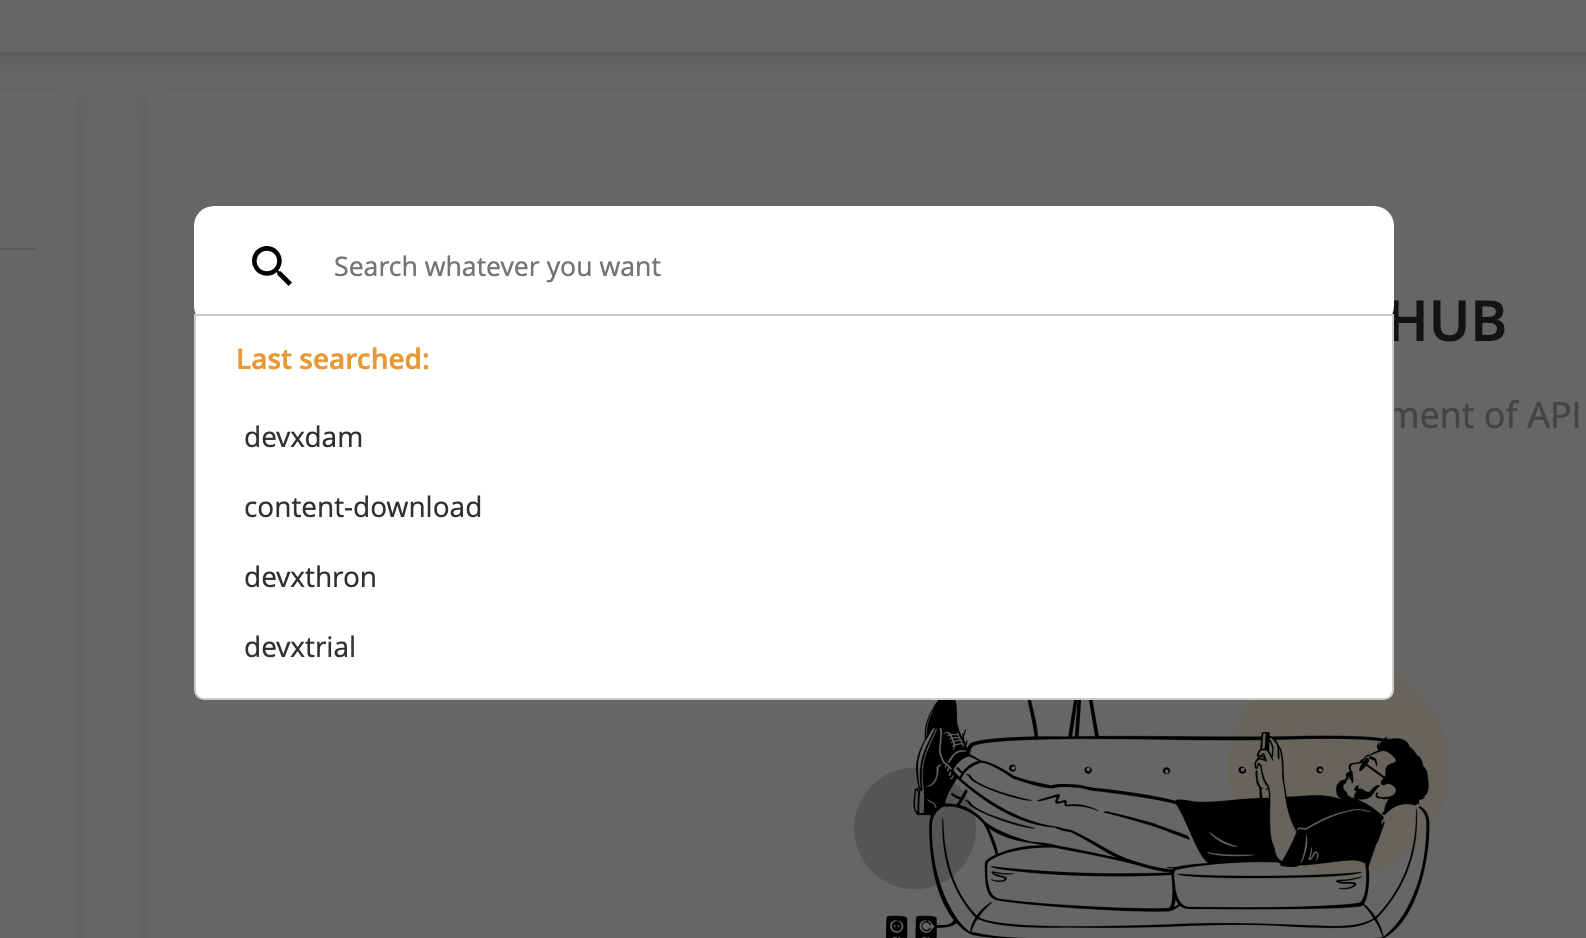
\includegraphics[width=0.6\textwidth, alt={Barra di ricerca globale dell'applicazione}]{images/frontend/SearchBar.jpg}
  \caption{SearchBar}\label{fig:search-bar}
\end{figure}
\pagebreak

\subsubsection{Autocomplete}\label{subsubsec:autocomplete}
Il componente rappresenta l'elenco dei risultati visualizzato sotto la barra di ricerca dell'applicazione (in figura~\ref{fig:autocomplete}).
Essa consiste in una lista di suggerimenti dinamici che vengono visualizzati in base al testo inserito dall'utente. 
In caso il campo di ricerca della \textit{SearchBar} sia vuoto, verrà mostrata la lista degli ultimi quattro termini cercati, se presenti.
In caso contrario, quando è presente un termine nella barra di ricerca, verrà visualizzata una lista di suggerimenti divisa per categoria.
Nel caso in cui la ricerca non abbia prodotto risultati, verrà visualizzato un messaggio di errore, gestito tramite il componente \textit{SnackBar} descritto in seguito.\\
La logica della ricerca è completamente sviluppata lato \textit{backend} per estrapolare il componente di ricerca e renderlo riutilizzabile in altri progetti.
Essendo un componente \textit{custom}, ho aggiunto la possibilità di navigare il menù e selezionare un suggerimento tramite tastiera, funzionalità 
obbligatoria per rendere la ricerca accessibile anche a persone con disabilità.\\
Dopo aver selezionato un suggerimento, verrà aperta la pagina di dettaglio dell'API corrispondente se l'utente ha scelto un'API specifica.  In caso contrario, il client-id corrente verrà impostato e la Chip verrà aggiornata.
Il componente infine supporta la gestione di più liste di elementi per la ricerca globale, non limitandosi a soli due elenchi. Questo significa che è possibile avere un numero variabile di liste di elementi con cui effettuare la ricerca globale. 

\begin{figure}[ht]
  \centering
  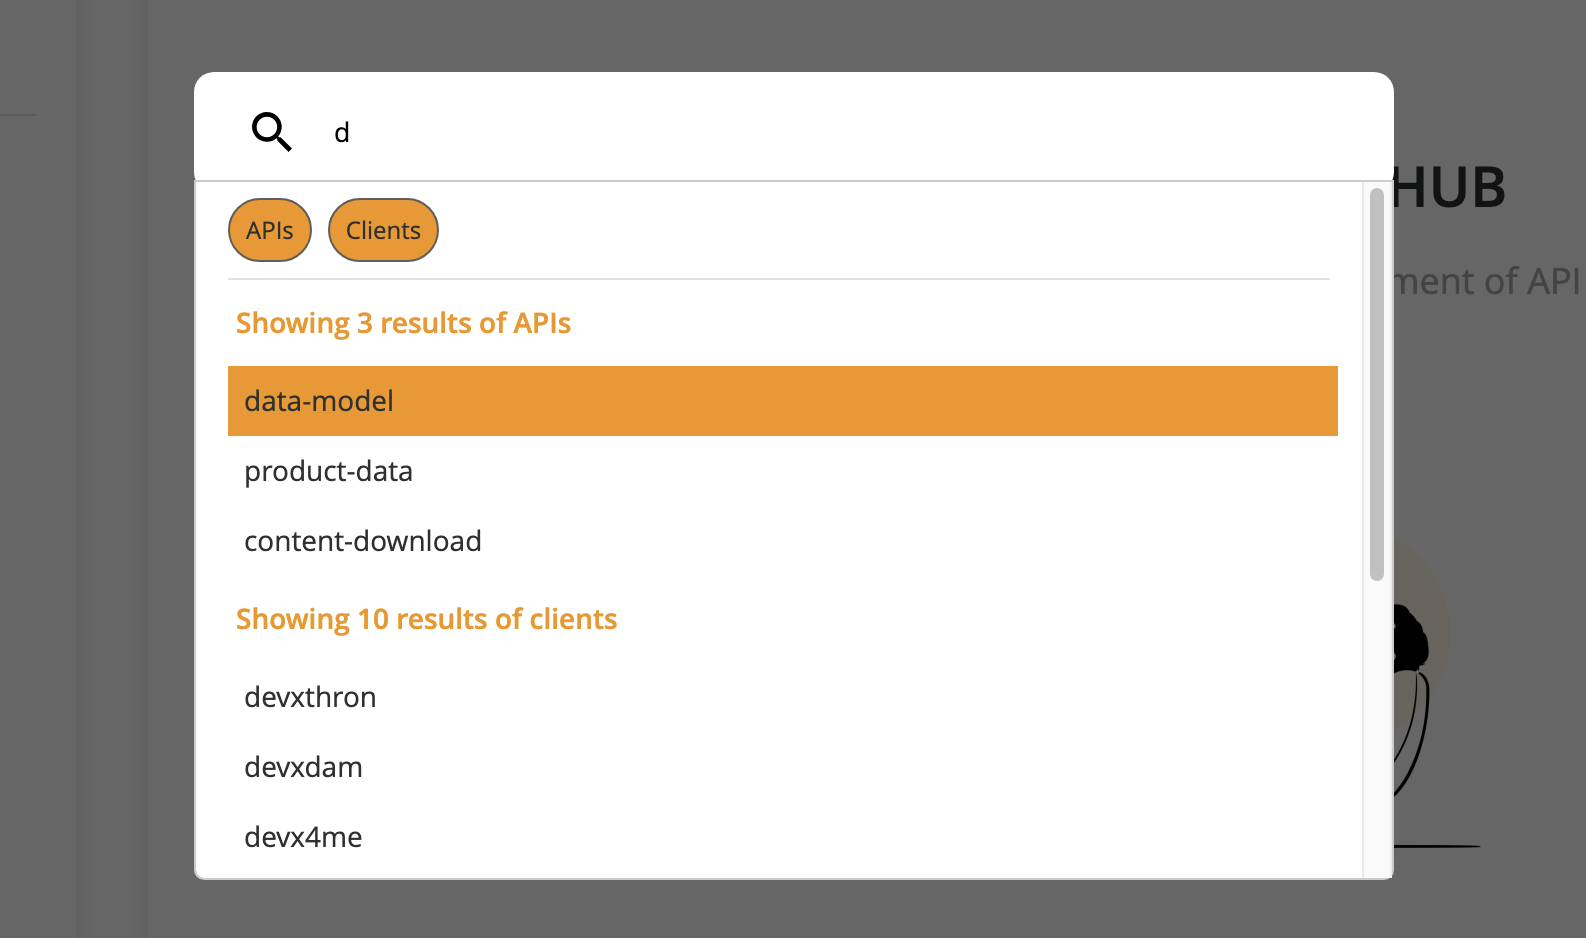
\includegraphics[width=0.6\textwidth, alt={Componente che si occupa della lista dinamica di risultati}]{images/frontend/SearchBar2.jpg}
  \caption{Autocomplete}\label{fig:autocomplete}
\end{figure}
\pagebreak
\subsubsection{Chip}\label{subsubsec:chip}
Il componente rappresenta la \textit{chip} situata nella barra di navigazione superiore dell'applicazione (in figura~\ref{fig:chip}).
Essa è utile a visualizzare il \textit{client-id} corrente, ovvero il \textit{client-id} che l'utente ha selezionato tramite la barra di ricerca globale.
Se l'utente non ha ancora effettuato alcuna selezione, verrà visualizzato il \textit{client-id} predefinito dell'ambiente di sviluppo.
Inoltre è possibile reimpostare il \textit{client-id} corrente cliccando sull'icona di reset a forma di \textit{X}, riportandolo al valore di default.
In caso il \textit{client-id} fosse già al valore predefinito, verrà visualizzato un messaggio di errore tramite il componente \textit{SnackBar} descritto in seguito.

\begin{figure}[ht]
  \centering
  
\includegraphics[width=0.3\textwidth, alt={Chip contenente il client id corrente}]{images/frontend/Chip.jpg}
  \caption{Chip}\label{fig:chip}
\end{figure}


\subsubsection{Filter}\label{subsubsec:filter}
Il componente rappresenta il bottone per filtrare la lista dei risultati della ricerca, all'interno del componente \textit{Autocomplete}.
Quando il bottone viene cliccato, lo sfondo risulta bianco e verrà visivamente nascosta la lista corrispondente al filtro cliccato.
Cliccando di nuovo sullo stesso filtro, il bottone tornerà arancione e verrà  mostrata la lista corrispondente al filtro cliccato.


\subsubsection{OptionList}\label{subsubsec:option-list}
Il componente rappresenta la lista di opzioni generiche, visualizzate all'interno della SideBar. Nel mio progetto, è stata utilizzata per visualizzare la lista
di tutte le \textit{API} disponibili nel sistema. 

\subsubsection{OptionListItem}\label{subsubsec:option-list-item}
Il componente rappresenta un singolo elemento della lista di opzioni generiche, visualizzate all'interno della SideBar. Nel mio progetto, un'\textit{item} rappresenta una singola \textit{API}.
Andando a cliccare un'opzione, verrà aperta la pagina di dettaglio dell'\textit{API} selezionata.

\subsubsection{SnackBar}\label{subsubsec:snack-bar}
Il componente rappresenta la \textit{snack-bar} dell'applicazione usata per la visualizzazione di messaggi di errore o di successo (in figura~\ref{fig:snack-bar}).
All'interno del portale è utilizzata per comunicare all'utente che un termine cercato non ha prodotto risultati, che il \textit{client-id} è stato resettato con successo
oppure per informare l'utente che il \textit{client-id} è già al valore di default.
Ho creato il componente con l'idea di renderlo riutilizzabile per diversi scopi, infatti è possibile modificare vari aspetti come il colore, il tipo di icona,
la durata del messaggio, il testo da visualizzare, la posizione del componente e la dimensione del componente.

\begin{figure}[ht]
  \centering
  
\includegraphics[width=0.5\textwidth, alt={Snackbar di errore}]{images/frontend/SnackBar1.jpg}
  \caption{SnackBar}\label{fig:snack-bar}
\end{figure}

\subsubsection{Loader}\label{subsubsec:loader}
Il seguente componente rapppresenta il sistema di caricamento principale dell'applicazione (in figura~\ref{fig:loader}).
Esso rappresenta un caricamento stile \textit{skeleton}, ovvero un caricamento che simula la presenza di contenuti, mentre questi vengono caricati, attraverso 
uno sfondo dinamico grigio.
Il componente è stato utilizzato per il caricamento della struttura della pagina, ovvero è composto da tre sezioni: \textit{HeaderNav}, \textit{SideBar} e
\textit{MainContent}. Il loader sarà visibile subito dopo aver effettuato il login o quando la pagina viene ricaricata, e scomparirà una volta che i dati saranno stati caricati correttamente.
Inoltre il componente è stato sviluppato utilizzando un design responsive, infatti seguirà la stessa struttura della pagina, andando a nascodere la sezione 
\textit{SideBar} in caso di schermi di piccole dimensioni.
Ho preferito utilizzare un caricamento di tipo \textit{skeleton} rispetto ad un classico \textit{loader} circolare, perchè secondo me migliora l'esperienza utente 
conferendo una sensazione migliore durante l'attesa del caricamento dei dati.

\begin{figure}[ht]
  \centering
  
\includegraphics[width=0.6\textwidth, alt={Skeleton loader di caricamento principale dell'applicazione}]{images/frontend/Loader.jpg}
  \caption{Loader}\label{fig:loader}
\end{figure}
\pagebreak

\section{Codifica backend}\label{sec:codifica-backend}

\subsection{Middleware}\label{subsec:middleware}
Il middleware è un meccanismo che permette di eseguire delle operazioni specifiche durante il ciclo di vita di una richiesta HTTP. 
Nel mio caso ho utilizzato questa funzionalità per svolgere della logica prima che la richiesta venga inoltrata al Controller e generi una risposta.
Il middleware è stato utilizzato per due scopi principali: la validazione del \textit{token JWT} di autenticazione e l'acquisizione del \textit{supertoken} utile per eseguire delle chiamate.
Basandoci sul ciclo di vita, il middleware intercetta le richieste, effettua le funzionalità appena descritte e successivamente inoltra la richiesta al Controller che si occuperà di restituire una risposta.
Quindi ogni chiamata verso gli \textit{endpoint} che ho sviluppato e che verranno descritti in seguito, passerà prima dal middleware. Questo perchè sono andato a specificare
nel modulo principale dell'applicazione le rotte che devono essere gestite dal \textit{middleware}, ovvero i controller di \textit{client-id}, \textit{API} e \textit{search}.

\subsubsection{Validazione token JWT}
La prima funzione implementata nel middleware è la validazione del \textit{token JWT} di autenticazione. Questa funzionalità è necessaria perchè all'interno del portale è presente un sistema di autenticazione, quindi sicuramente le chiamate verso i servizi \textit{backend} creati sono protetti dal login del portale.
La criticità consiste nel fatto che un servizio può essere accessibile direttamente, senza la necessità di passare attraverso il portale, poiché ciascun endpoint dispone di un URL pubblico.
La soluzione che sono andato ad adottare è stata quella di validare il token di autenticazione verificando che qualsiasi chiamata ai miei servizi fosse effettuata da un utente autenticato, avente un token valido nell'\textit{header} della richiesta.
Per verificare il \textit{token} ho effettuato i seguenti passaggi:
\begin{enumerate}
  \item Verifico che il \textit{token} di autenticazione sia presente nell'\textit{header} della richiesta. In caso non lo sia viene restituito un errore 401;
  \item Il \textit{token} viene decodificato e viene salvato solo l'\textit{header} di esso. In caso il risultato salvato non sia valido, viene restituito un errore 401;
  \item Vado ad estrarre il campo \textit{KID}, che identifica quale chiave pubblica verrà utilizzata per la verifica;
  \item Eseguo una \textit{GET} verso l'\textit{endpoint} di \textit{Microsoft AAD} per ottenere le informazioni di configurazione di \textit{OpenID Connect} (OIDC). 
  Queste informazioni includono gli \textit{url} da dove è possibile ottenere le chiavi pubbliche per la verifica del \textit{token};
  \item Vado ad estrarre l'\textit{url} che specifica dove trovare le chiavi pubbliche \textit{JSON Web Key Set} (JWKS) e faccio una seconda \textit{GET} verso l'\textit{endpoint} appena descritto;
  \item Effettuo un controllo con la chiave pubblica corrispondente all'intestazione del token JWT (identificata dal campo `\textit{kid}') nell'elenco delle chiavi ottenute da \textit{Azure AD}. Nel caso di nessuna corrispondenza viene restituito un errore 401;
  \item La chiave pubblica viene convertita e formattata in un certificato \textit{X509} valido;
  \item Effettuo la validazione del \textit{token} utilizzando la chiave pubblica convertita. Il risultato conterrà il \textit{payload} del \textit{token JWT} se la verifica ha successo o genererà un errore se la verifica fallisce.
\end{enumerate}

\subsubsection{GET Supertoken}
La seconda funzione implementata nel \textit{middleware} è l'acquisizione del \textit{supertoken}, che avviene solamente se la validazione del \textit{token} appena discussa non genera errori.
Per ottenere il \textit{supertoken} è necessario effettuare una chiamata verso un \textit{endpoint} aziendale, che restituisce il \textit{supertoken} in base al \textit{client-id} passato come parametro.
Per prima cosa sono andato a creare dei parametri, aggiungendo l'\textit{username} con il valore che mi è stato fornito dall'azienda.
Successivamente vado ad effettuare una \textit{POST} verso l'\textit{endpoint} aziendale che mi ritorna il \textit{supertoken}, e in caso di criticità viene restituito un errore.\\
Il \textit{token} appena ottenuto viene aggiunto all'\textit{header} della richiesta, in modo tale che ogni chiamata verso i miei \textit{endpoint}, avrà il \textit{supertoken} aggiunto automaticamente.

% Forse da aggiungere in architettura progettazione

\subsection{Endpoints}\label{subsec:endpoints}
La seguente sezione descrive gli \textit{endpoint} che ho creato all'interno del mio progetto. Tutti gli \textit{endpoint} sviluppati 
sono utilizzati all'interno del progetto \textit{frontend} descritto in precedenza.
Come descritto nel capitolo dell'architettura (in sezione~\ref{subsec:architettura-backend}), ogni endpoint creato sarà formato da un \textit{Module}, un \textit{Controller} e un \textit{Service}.

\subsubsection{Client-id}
L'\textit{endpoint} rappresenta il punto di accesso per ottenere la lista dei \textit{client-id} disponibili nel sistema.
È definito dal file \textit{Module}, dove al suo interno vengono specificati i vari \textit{controller} e \textit{service} utilizzati.
Nel \textit{Controller} è presente l'endpoint `\textit{/clients}', ovvero un metodo \textit{GET} che restituisce la lista dei \textit{client-id} andando
a chiamare il metodo `\textit{getAllClients}' del \textit{Service}.
All’interno del metodo appena citato, viene chiamato un altro endpoint sviluppato dall'azienda, che restituisce 
la lista dei \textit{client-id} disponibili per l'ambiente di sviluppo in cui ci si trova.
Per chiamare questo \textit{endpoint}, sono state configurate all'interno dell'applicativo le variabili d'ambiente.
Inoltre la chiamata necessita del \textit{supertoken}, che grazie al \textit{middleware} sarà aggiunto automaticamente all'interno 
dell'\textit{header} della chiamata.
Il metodo ritorna un \textit{array} di stringhe, dove ogni stringa rappresenta un \textit{client-id} disponibile nel sistema.

\subsubsection{API}
L'\textit{endpoint} rappresenta il punto di accesso per ottenere la lista di \textit{API} disponibili nel sistema.
È definito dal file \textit{Module}, dove al suo interno vengono specificati i vari \textit{controller} e \textit{service} utilizzati.
Nel \textit{Controller} è presente l'endpoint `\textit{/apis}', ovvero un metodo \textit{GET} che restituisce la lista delle \textit{API} andando
a chiamare il metodo `\textit{getAllApis}' del \textit{Service}.
All'interno del metodo appena citato, è presente la logica necessaria per restituire la lista completa di \textit{API} disponibili, che poi sarà visibile nel portale.
Il metodo utilizza un endpoint aziendale per ottenere la lista di \textit{API} dei servizi THRON.
Il metodo restituisce un \textit{array} di oggetti, dove ogni oggetto è rappresentato dal nome del servizio e dall'\textit{url} corrispondente.

\subsubsection{Search}
L'\textit{endpoint} rappresenta il punto di accesso per ottenere la lista di suggerimenti utilizzata per la ricerca globale del portale.
È definito dal file \textit{Module}, dove al suo interno vengono specificati i vari \textit{controller}, \textit{service} e gli \textit{imports} utilizzati. 
Quest'ultimi non sono altro che dei moduli che vengono utilizzati all'interno del \textit{controller}. Nel mio caso sono andato ad importare il modulo \textit{APIModule}
relativo alle \textit{API} e il modulo \textit{ClientModule} relativo ai \textit{client-id}.
Nel \textit{Controller} è presente l'endpoint `\textit{/results}', ovvero un metodo \textit{POST} che restituisce la lista di suggerimenti in base ad un parametro di ricerca
inserito nel \textit{body} della chiamata. Il metodo in primis ottiene le \textit{API} e i \textit{client-id} utilizzando i moduli importati. 
Successivamente viene chiamato il metodo `\textit{getResults}' del \textit{Service}, al quale vengono passati come parametri il termine di ricerca, la lista delle \textit{API} e la lista dei \textit{client-id}.
All'interno della funziona appena citata, è presente tutta la logica di filtraggio dei risultati. In precedenza tutta la logica era gestita lato \textit{frontend}, ma successivamente 
è stata spostata lato \textit{backend} per estrapolare la logica e renderla riutilizzabile in altri progetti, andando così a rispettare una \textit{best practice} aziendale.
Il servizio che ho creato va a restituire una lista di risultati, dove ogni risultato è un oggetto che contiene il nome del gruppo filtrato con la lista associata al gruppo.
Inoltre ho impostato un limite di risultati, infatti la chiamata andrà a restituire al massimo dieci risultati per ogni gruppo, evitando di avere una lista troppo lunga di risultati che risulterebbe difficile 
da visualizzare.
